\documentclass{report}

\usepackage[T2A]{fontenc}
\usepackage[utf8]{luainputenc}
\usepackage[english, russian]{babel}
\usepackage[pdftex]{hyperref}
\usepackage[14pt]{extsizes}
\usepackage{listings}
\usepackage{color}
\usepackage{geometry}
\usepackage{enumitem}
\usepackage{multirow}
\usepackage{graphicx}
\usepackage{indentfirst}
\usepackage{float}

\geometry{a4paper,top=2cm,bottom=3cm,left=2cm,right=1.5cm}
\setlength{\parskip}{0.5cm}
\setlist{nolistsep, itemsep=0.3cm,parsep=0pt}

\lstset{language=C++,
		basicstyle=\footnotesize,
		keywordstyle=\color{blue}\ttfamily,
		stringstyle=\color{red}\ttfamily,
		commentstyle=\color{green}\ttfamily,
		morecomment=[l][\color{magenta}]{\#}, 
		tabsize=4,
		breaklines=true,
  		breakatwhitespace=true,
  		title=\lstname,       
}

\makeatletter
\renewcommand\@biblabel[1]{#1.\hfil}
\makeatother

\begin{document}

\begin{titlepage}

\begin{center}
Министерство науки и высшего образования Российской Федерации
\end{center}

\begin{center}
Федеральное государственное автономное образовательное учреждение высшего образования \\
Национальный исследовательский Нижегородский государственный университет им. Н.И. Лобачевского
\end{center}

\begin{center}
Институт информационных технологий, математики и механики
\end{center}

\vspace{4em}

\begin{center}
\textbf{\LargeОтчет по лабораторной работе} \\
\end{center}
\begin{center}
\textbf{\Large«Построение выпуклой оболочки для компонент бинарного изображения»} \\
\end{center}

\vspace{4em}

\newbox{\lbox}
\savebox{\lbox}{\hbox{text}}
\newlength{\maxl}
\setlength{\maxl}{\wd\lbox}
\hfill\parbox{7cm}{
\hspace*{5cm}\hspace*{-5cm}\textbf{Выполнил:} \\ студент группы 381808-1 \\ Еремина Алёна\\
\\
\hspace*{5cm}\hspace*{-5cm}\textbf{Проверил:}\\ доцент кафедры МОСТ, \\ кандидат технических наук \\ Сысоев А.В.\\
}
\vspace{\fill}

\begin{center} Нижний Новгород \\ 2021 \end{center}

\end{titlepage}

\setcounter{page}{2}

% Введение
\section*{Введение}
\addcontentsline{toc}{section}{Введение}
Построение выпуклой оболочки для компонент бинарного изображения - важная задача в области компьютерного зрения. Эта задача делится на две части: разбиение бинарного изображения на компоненты и построение минимальной выпуклой оболочки для каждой компоненты.
\newpage

% Постановка задачи
\section*{Постановка задачи}
\addcontentsline{toc}{section}{Постановка задачи}
В данной работе необходимо реализовать построение выпуклой оболочки для компонент бинарного изображения. Данная работа должна содержать последовательную и две параллельных реализации с использованием технологий OpenMP и TBB. 
\par
На основе разработанных реализаций необходимо провести качественное сравнение изображений, полученных разными реализациями алгоритма, и вычислительные эксперименты, сравнив время работы последовательного и параллельных алгоритмов на разных входных изображениях, затем сделать вывод об эффективности параллельных версий.
\newpage

% Описание алгоритма
\section*{Описание алгоритма}
\addcontentsline{toc}{section}{Описание алгоритма}
Первая часть алгоритма простроения выпуклой оболочки для компонент бинарного изображения состоит в разбиении бинарного изображения на компоненты. Идея данного алгоритма основана на использовании уголка — ABC-маски, которая показана на рисунке 1. 
\begin{figure}[H]
\center{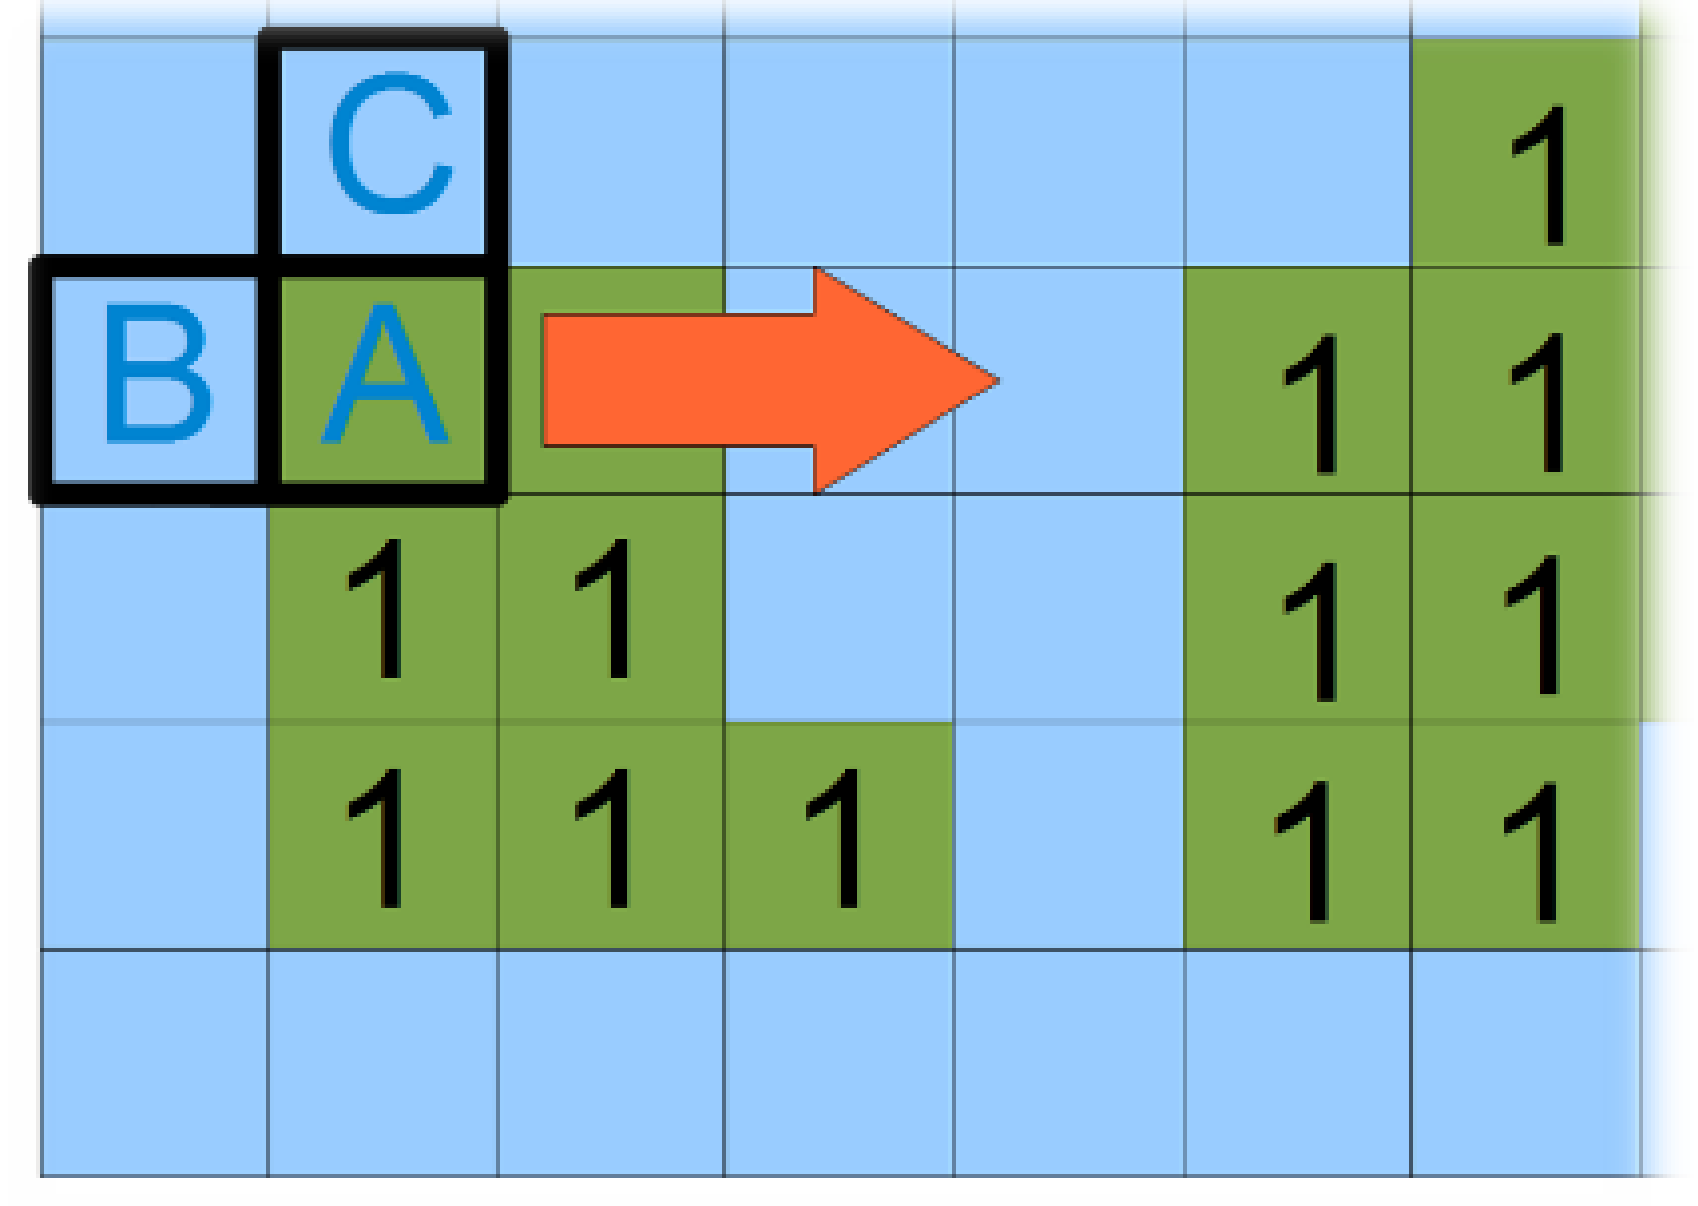
\includegraphics[scale=0.8]{./eremina_img/abc-mask1.pdf}}
\caption{ABC маска и направление сканирования изображения}
\end{figure}
Проход по изображению данной маской осуществляется слева-направо и сверху-вниз. Считается, что за границей изображения объектов нет, поэтому, если туда попадают B или C — это требует дополнительной проверки при сканировании. На рисунке 2 изображены 5 возможных позиций маски на изображении.
\begin{figure}[H]
\center{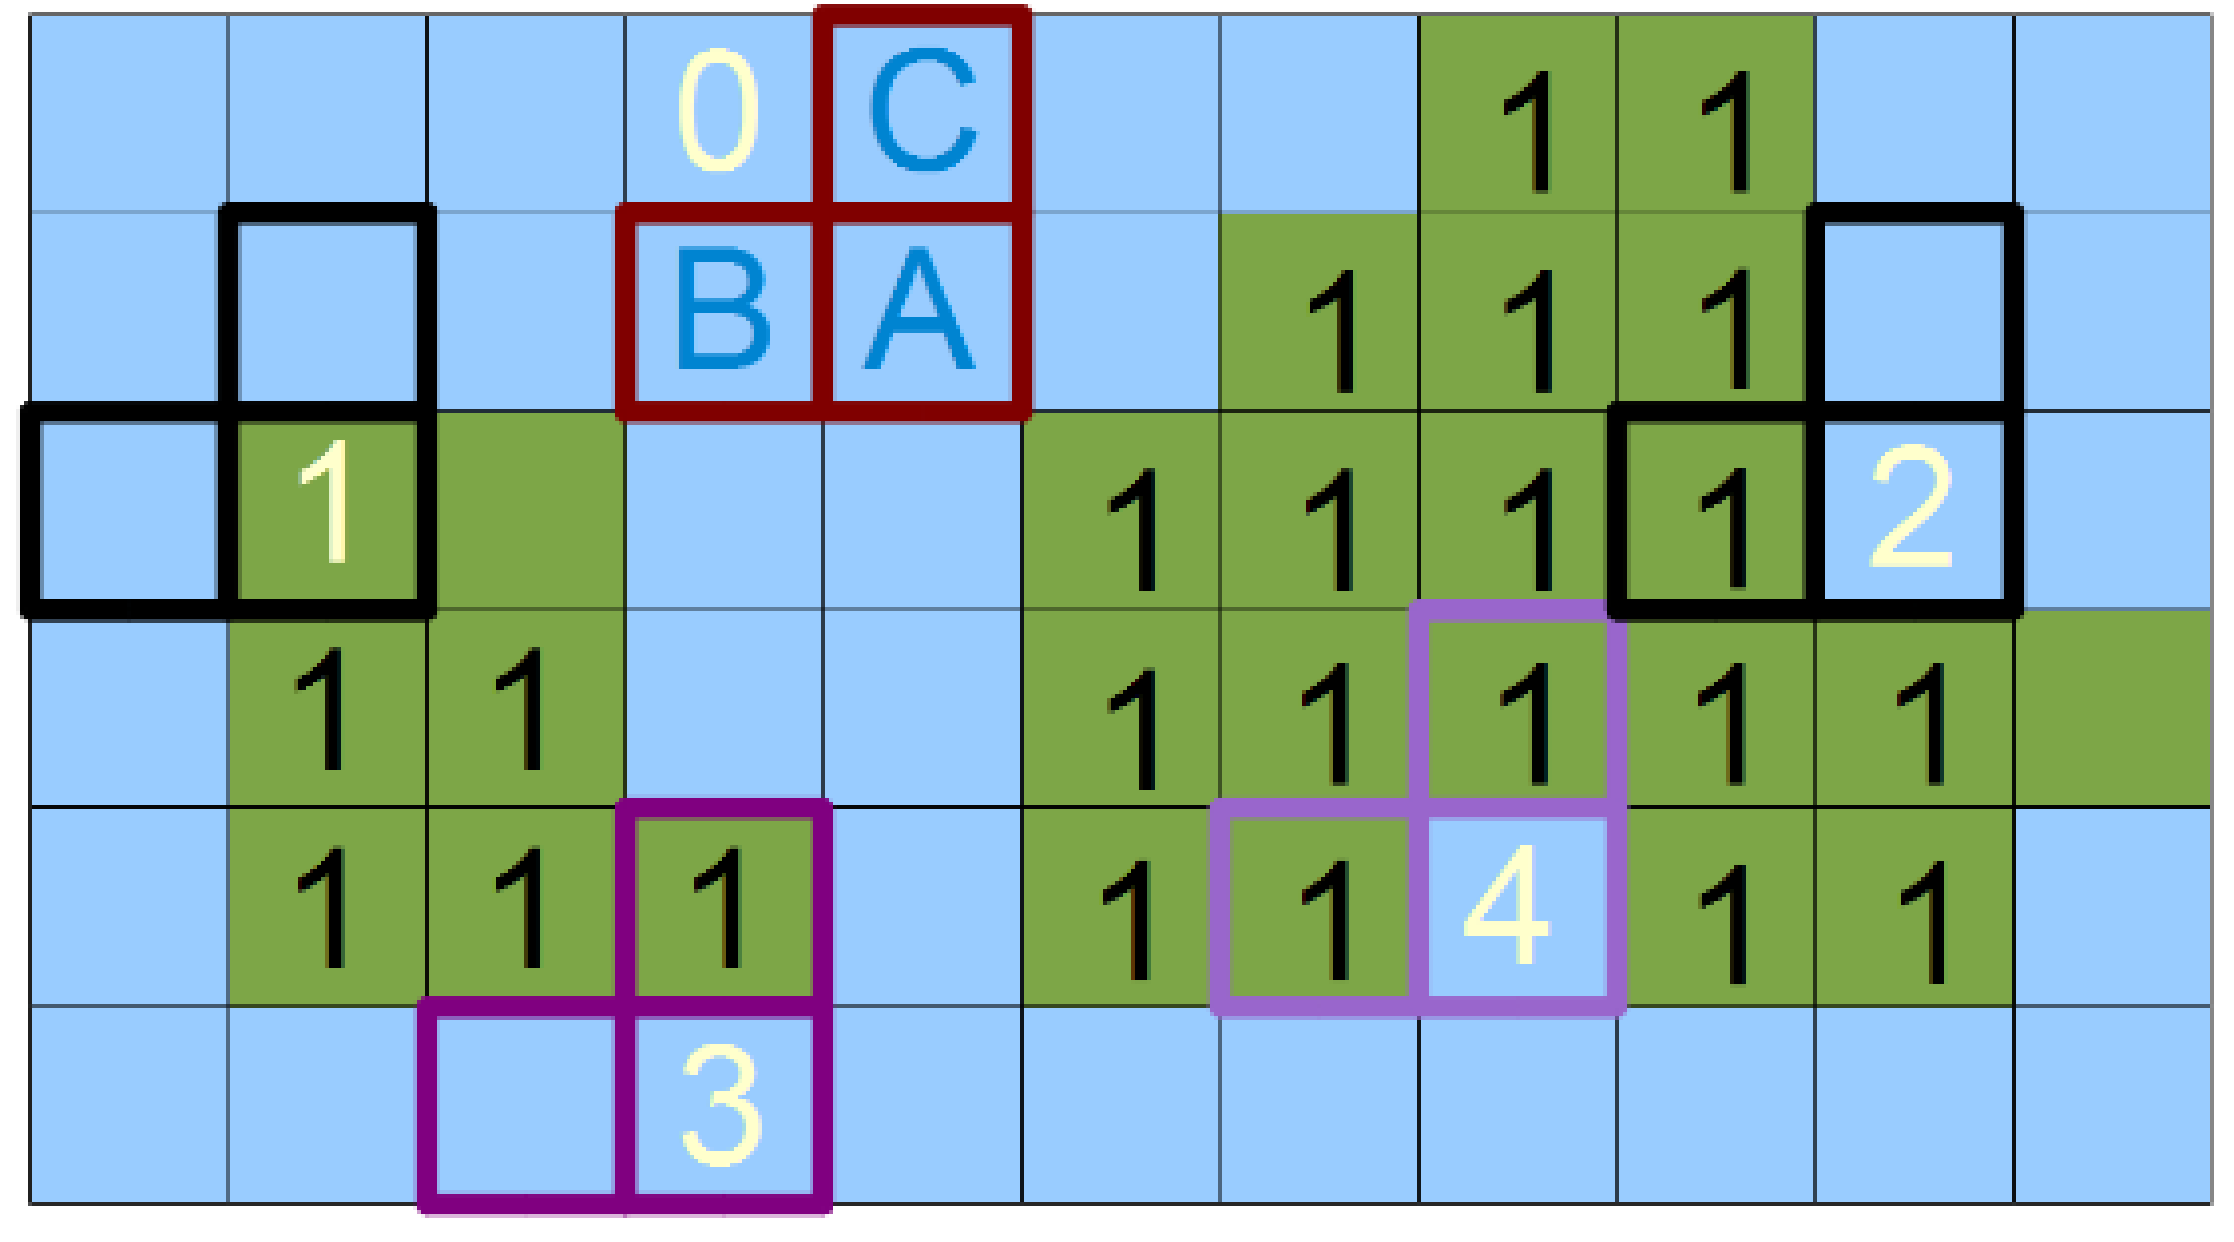
\includegraphics[scale=0.8]{./eremina_img/abc-mask2.pdf}}
\caption{Пять возможных позиций ABC-маски}
\end{figure}

\begin{enumerate}
	\item Позиция под номером 0, когда не размечены все три компонента маски — в этом случае мы просто пропускаем пиксель.
	\item Позиция под номером 1, когда помечен только элемент A — в этом случае мы говорим о создании нового объекта — новый номер.
	\item Позиция под номером 2, когда помечен элемент элемент B — в этом случае мы помечаем текущий пиксель A меткой, расположенной в B.
	\item Позиция под номером 3, когда помечен элемент элемент С — в этом случае мы помечаем текущий пиксель A меткой, расположенной в С.
	\item Позиция под номером 4, тогда мы говорим о том, что метки (номера объектов) B и C связаны — то есть эквивалентны и пиксель A может быть помечен либо как B либо как C. В некоторых реализация составляют граф эквивалентности таких меток, с последующим его разбором, однако на мой взгляд в это нет необходимости. Мы будем делать так — в том случае, если B не равно C то перенумеруем все уже обработанные пиксели помеченные как С в метку B. Но об этом в самом конце.
\end{enumerate}

\par
Следующий этап - построение выпуклой оболочки для каждой компоненты. Для решения этой задачи был реализован алгоритм Грэхема. В этом алгоритме задача о выпуклой оболочке решается с помощью стека, сформированного из точек-кандидатов. Все точки входного множества заносятся в стек, а потом точки, не являющиеся вершинами выпуклой оболочки, со временем удаляются из него. По завершении работы алгоритма в стеке остаются только вершины оболочки в порядке их обхода против часовой стрелки.
\par
Ниже приведён псевдокод данного алгоритма. В качестве входных данных выступает множество точек Q, где  |Q| >= 3. В ней вызывается функция Top(S), которая возвращает точку, находящуюся на вершине стека S, не изменяя при этом его содержимое. Кроме того, используется также функция NextToTop(S), которая возвращает точку, расположенную в стеке S, на одну позицию ниже от верхней точки; стек S при этом не изменяется.

Graham(Q)
\begin{enumerate}
	\item Пусть p0 — точка из множества Q с минимальной координатой y или самая левая из таких точек при наличии совпадений
	\item Пусть <p1, p2, ... ,pm> — остальные точки множества Q, отсортированные в порядке возрастания полярного угла,измеряемого против часовой стрелки относительно точки p0 (если полярные углы нескольких точек совпадают, то по расстоянию до точки p0)
	\item Push(p0,S)
	\item Push(p1,S)
	\item for i = 2 to m do
	\item   while угол, образованный точками NextToTop(S),Top(S) и pi, образуют не левый поворот(при движении по ломаной, образованной этими точками, мы движемся прямо или вправо)
	\item      do Pop(S)
	\item    Push(pi,S)
	\item return S
\end{enumerate}

\newpage

% Схема распараллеливания
\section*{Схема распараллеливания}
\addcontentsline{toc}{section}{Схема распараллеливания}
После того, как изображения было поделено на компоненты, каждая компонента записывается в собственный буфер, размер которого зависит от размера компопенты. Далее каждый буфер с компонентой обрабатывается отдельными потоками. В конце, каждый поток по очереди записывает результат своей работы (выпуклая оболочка) в результирующее изображение
\newpage

% Описание программной реализации
\section*{Описание программной реализации}
\addcontentsline{toc}{section}{Описание программной реализации}
В программе имеются следующие функции:

\begin{itemize}
\item Разбиение бинарного изображения на компоненты
\end{itemize}
\begin{lstlisting}
	std::map<int, int> splitImageIntoComponents(std::vector<int>* img_src_dst, const int width, const int height);
\end{lstlisting}
\begin{itemize}
\item Функция сортировки точек в порядке возрастания полярного угла, измеряемого против часовой стрелки относительно точки p0 
\end{itemize}
\begin{lstlisting}
	void sortPolar(point* points, const point* p0, const int count);
\end{lstlisting}
\begin{itemize}
\item Функция, проверяющая, образуют ли точки a, b и c правый повотор
\end{itemize}
\begin{lstlisting}
	  bool rightTurn(const point* a, const point* b, const point* c, bool flag);
\end{lstlisting}
\begin{itemize}
\item Функция, реализующая последовательную версию построения выпоклой оболочки для компонент бинарного изображения: 
\end{itemize}
\begin{lstlisting}
	std::vector<uint8_t> Convex_Hull(std::vector<uint8_t> img_src, const int height, const int width);
\end{lstlisting}
\begin{itemize}
\item Функция, реализующая OMP версию построения выпоклой оболочки для компонент бинарного изображения: 
\end{itemize}
\begin{lstlisting}
	std::vector<uint8_t> Convex_Hull_OMP(std::vector<uint8_t> img_src,const int height, const int width);
\end{lstlisting}
\begin{itemize}
\item Функция, реализующая TBB версию построения выпоклой оболочки для компонент бинарного изображения: 
\end{itemize}
\begin{lstlisting}
	std::vector<uint8_t> Convex_Hull_TBB(std::vector<uint8_t> img_src,const int height, const int width);
\end{lstlisting}
\newpage

% Описание экспериментов
\section*{Описание экспериментов}
\addcontentsline{toc}{section}{Описание экспериментов}
Эксперименты проводились на 4-х ядерном компьютере с операционной системой – Windows 10, который имеет 8 логических процессоров. Результаты экспериментов приведены в таблице:
\begin{table}[!h]
\caption{Результаты вычислительных экспериментов}
\centering
\begin{tabular}{llllll}
Размер (px) & Количество потоков & Seq & OMP & TBB \\
128x128 & 4 & 0.0316076 & 0.023816 & 0.0242111\\
256x256 & 4 & 0.279995 & 0.134528 & 0.093895\\
800x500 & 4 & 9.3129 & 5.82032 & 6.91643\\
1450x1000 & 4 & 93.2804 & 53.3695 & 57.6741\\
\end{tabular}
\end{table}
\par
По результатам экспериментов можно сделать вывод о том, что параллельные версии работают быстрее последовательной приверно в 1.5-2 раза. При этом, разница в производительности OMP и TBB не велика, что естественно, потому что схема распараллеливания одна и та же.
\par
Ниже привидены картинки, на которых производился вычислительный элемент. Первая картинка - исходое бинарное изображение, содержащее несколько компонент, вторая - результат последовательного алгоритма, третья - OMP реализация и четвёртая - TBB реализация. 

\begin{figure}[H]
\center{
\includegraphics[scale=1.2]{./eremina_img/128.pdf}}
\caption{Бинарное изображение 128x128}
\end{figure}

\begin{figure}[H]
\center{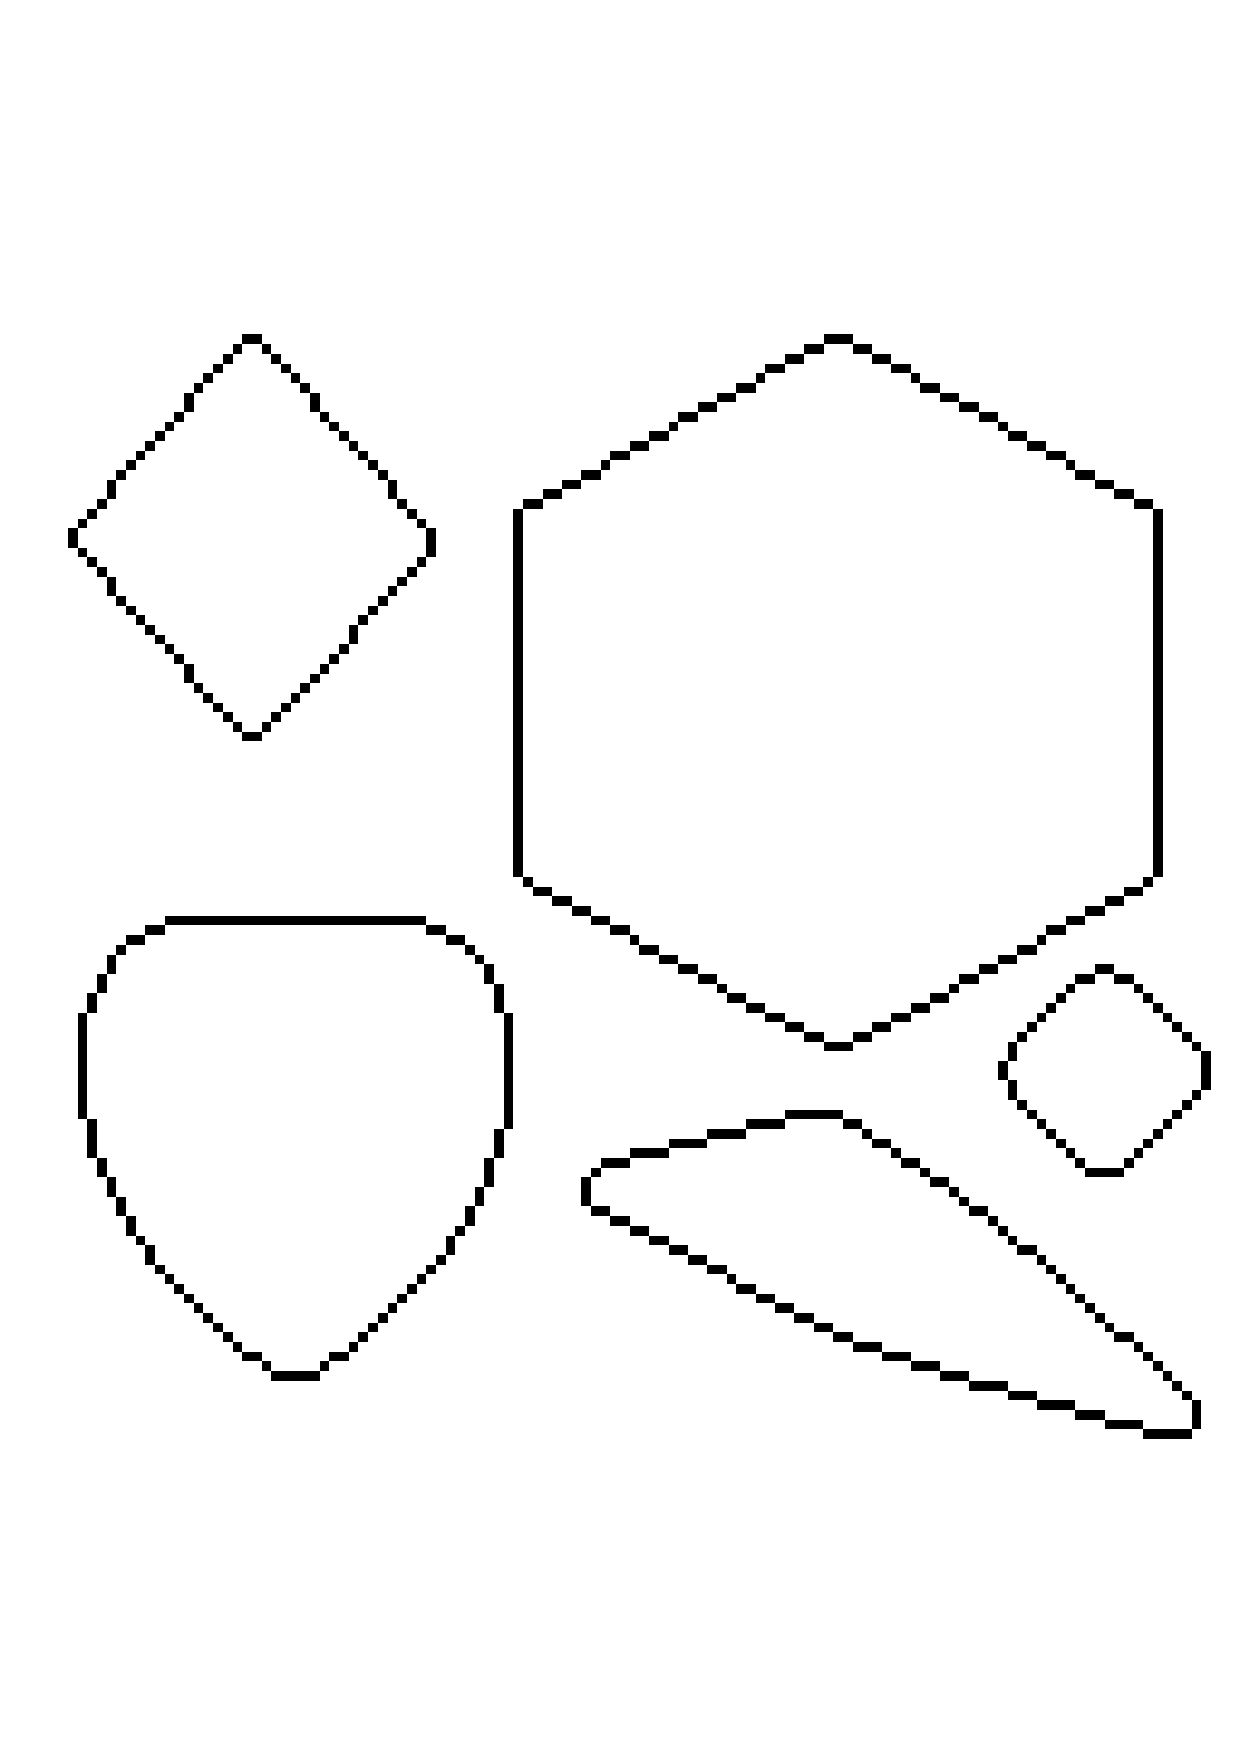
\includegraphics[scale=1.2]{./eremina_img/seq128.pdf}}
\caption{Последовательная реализация 128x128}
\end{figure}

\begin{figure}[H]
\center{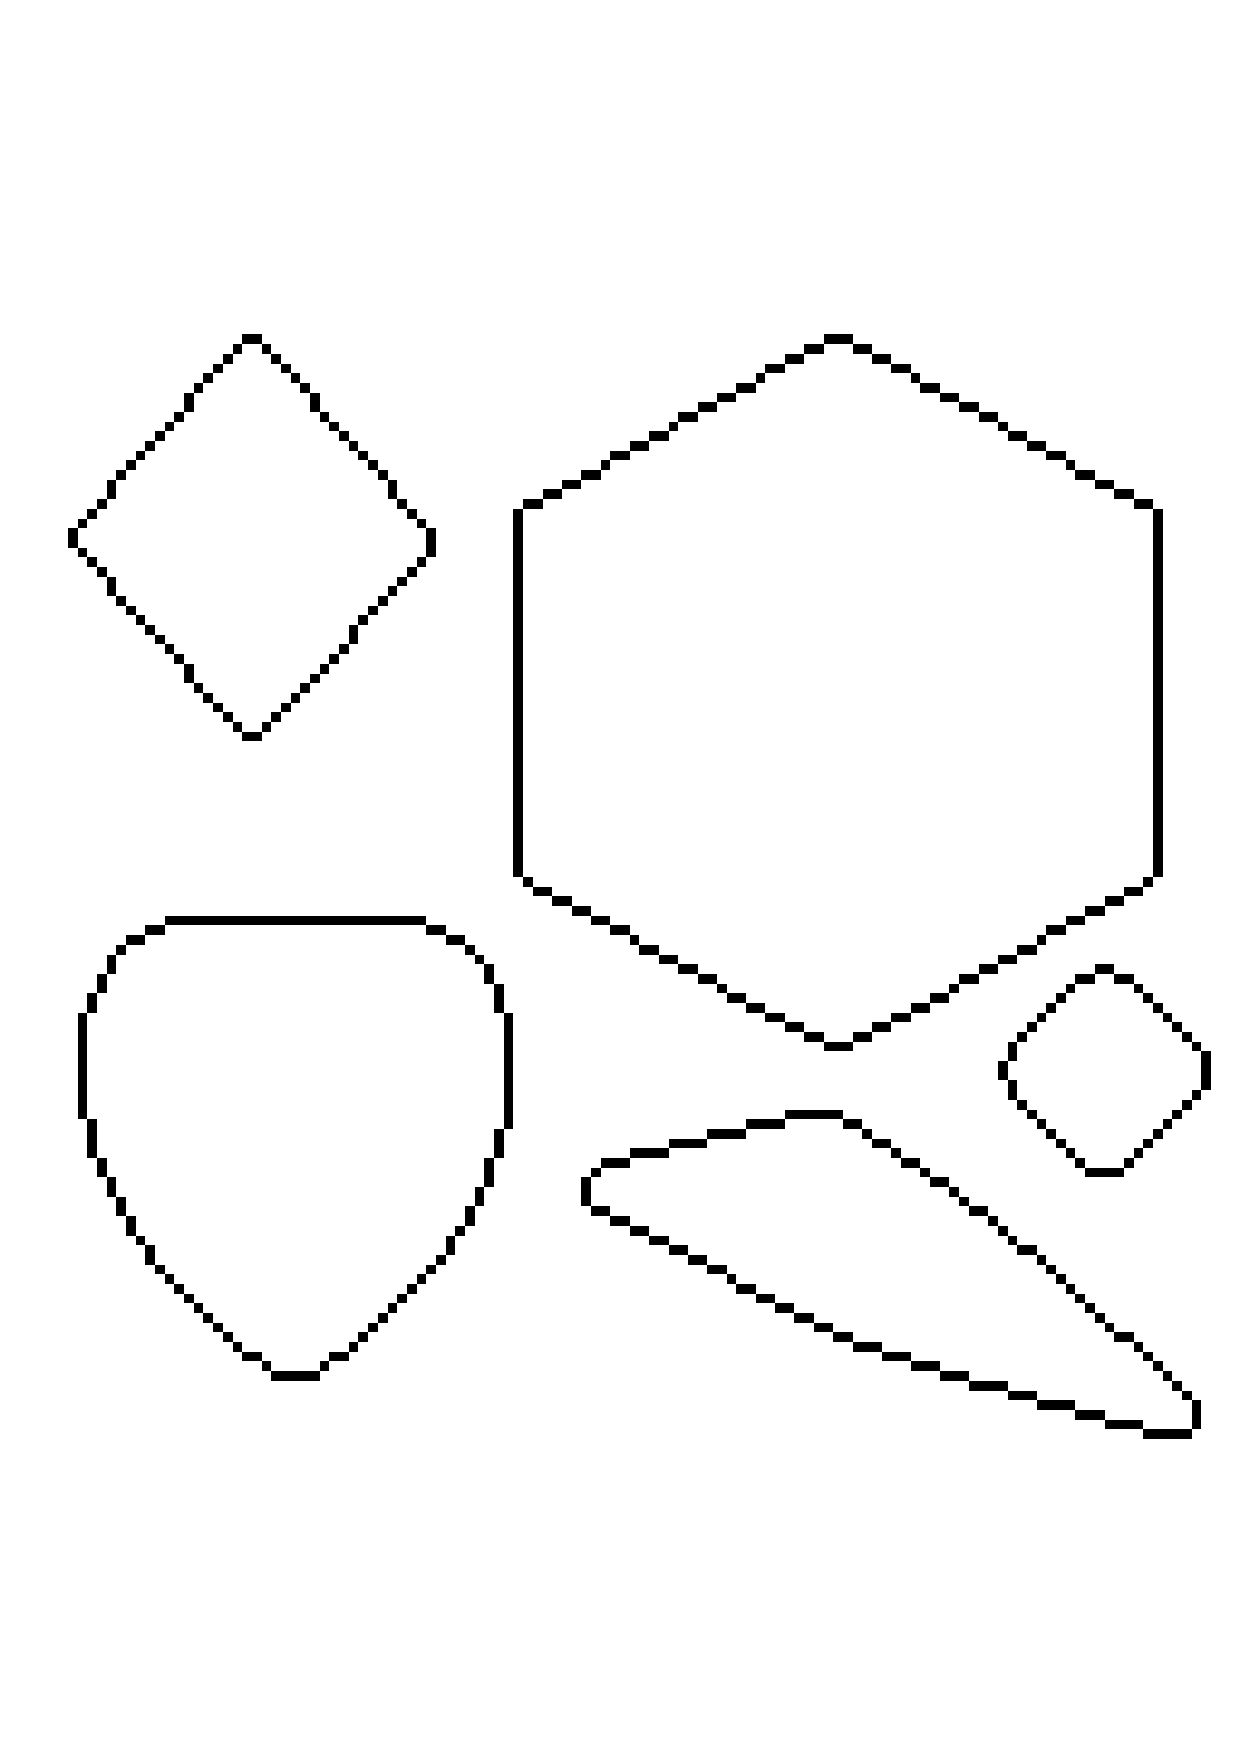
\includegraphics[scale=1.2]{./eremina_img/omp128.pdf}}
\caption{OMP реализация 128x128}
\end{figure}

\begin{figure}[H]
\center{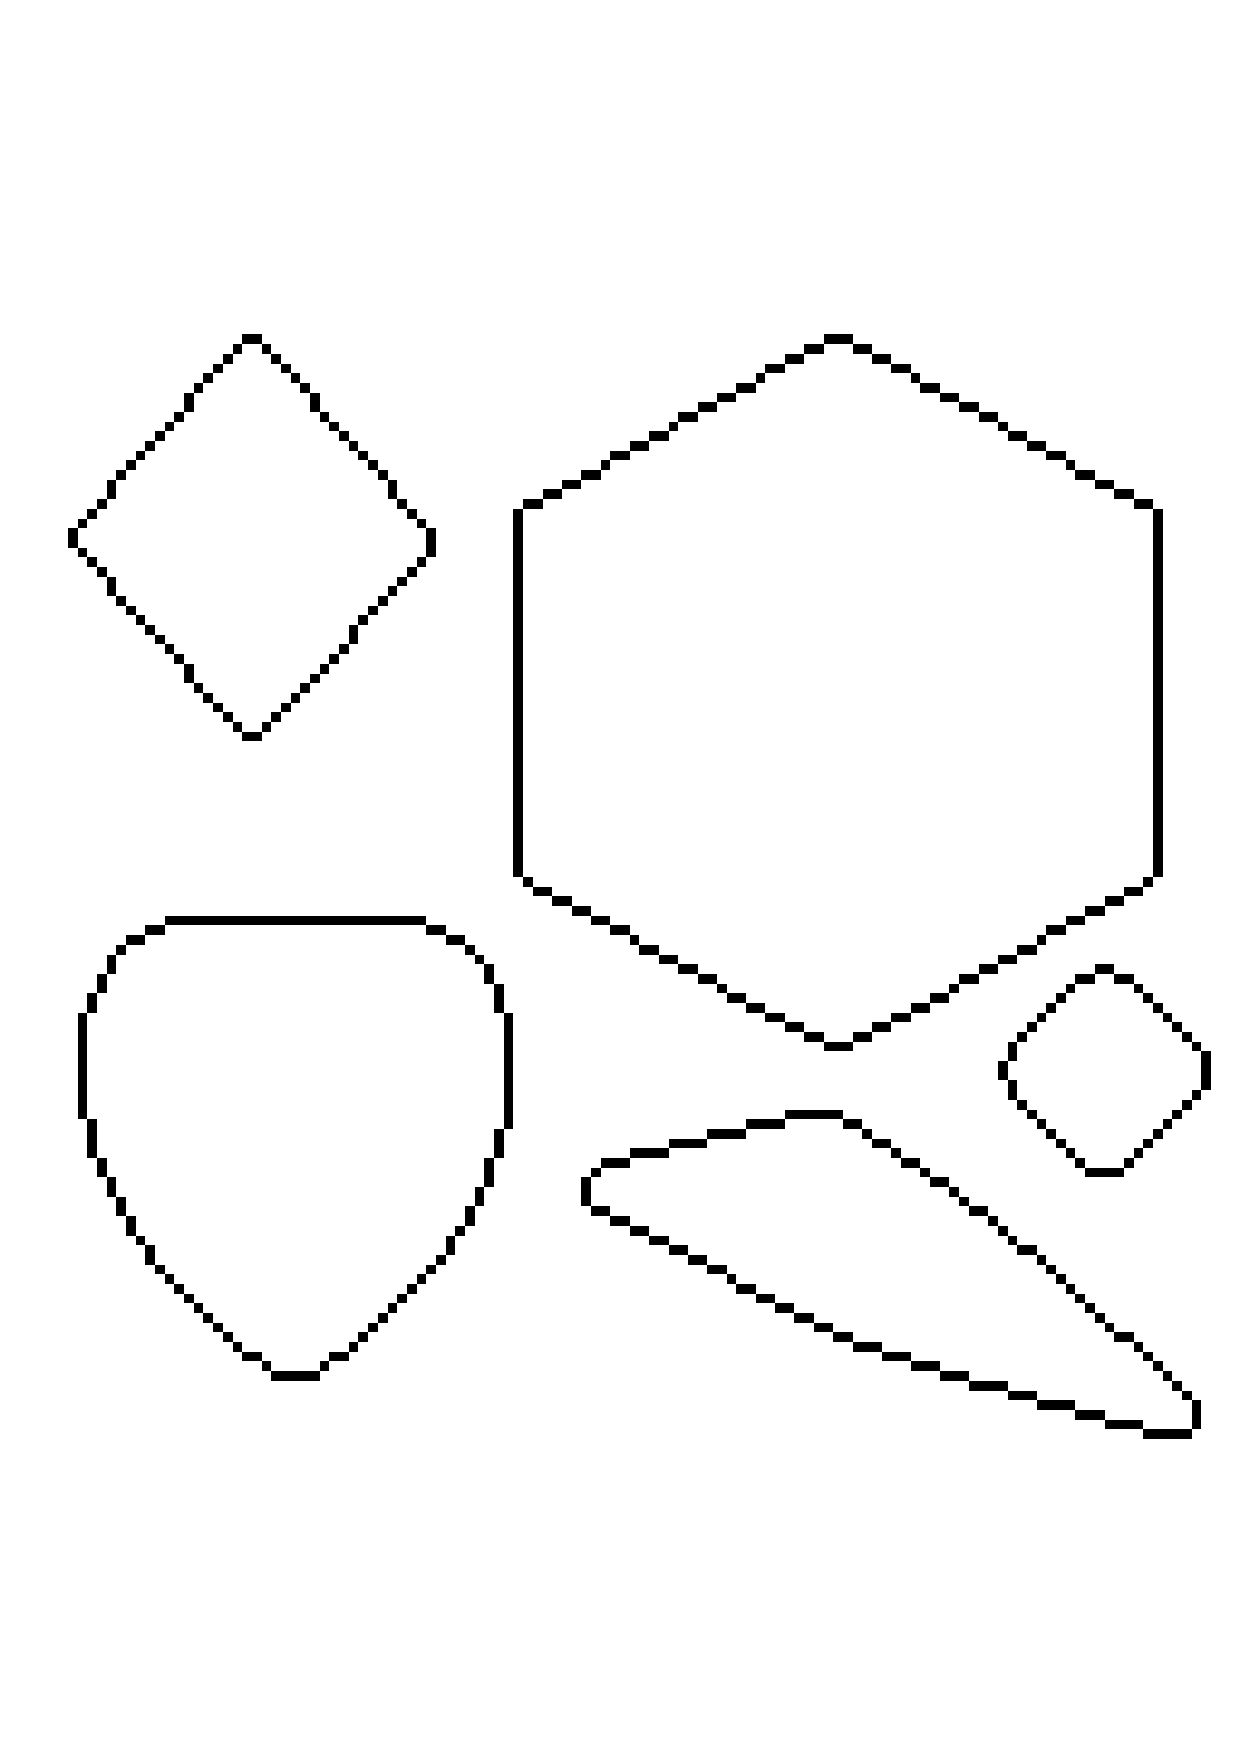
\includegraphics[scale=1.2]{./eremina_img/tbb128.pdf}}
\caption{TBB реализация 128x128}
\end{figure}

\begin{figure}[H]
\center{
\includegraphics[scale=1]{./eremina_img/256.pdf}}
\caption{Бинарное изображение 256x256}
\end{figure}

\begin{figure}[H]
\center{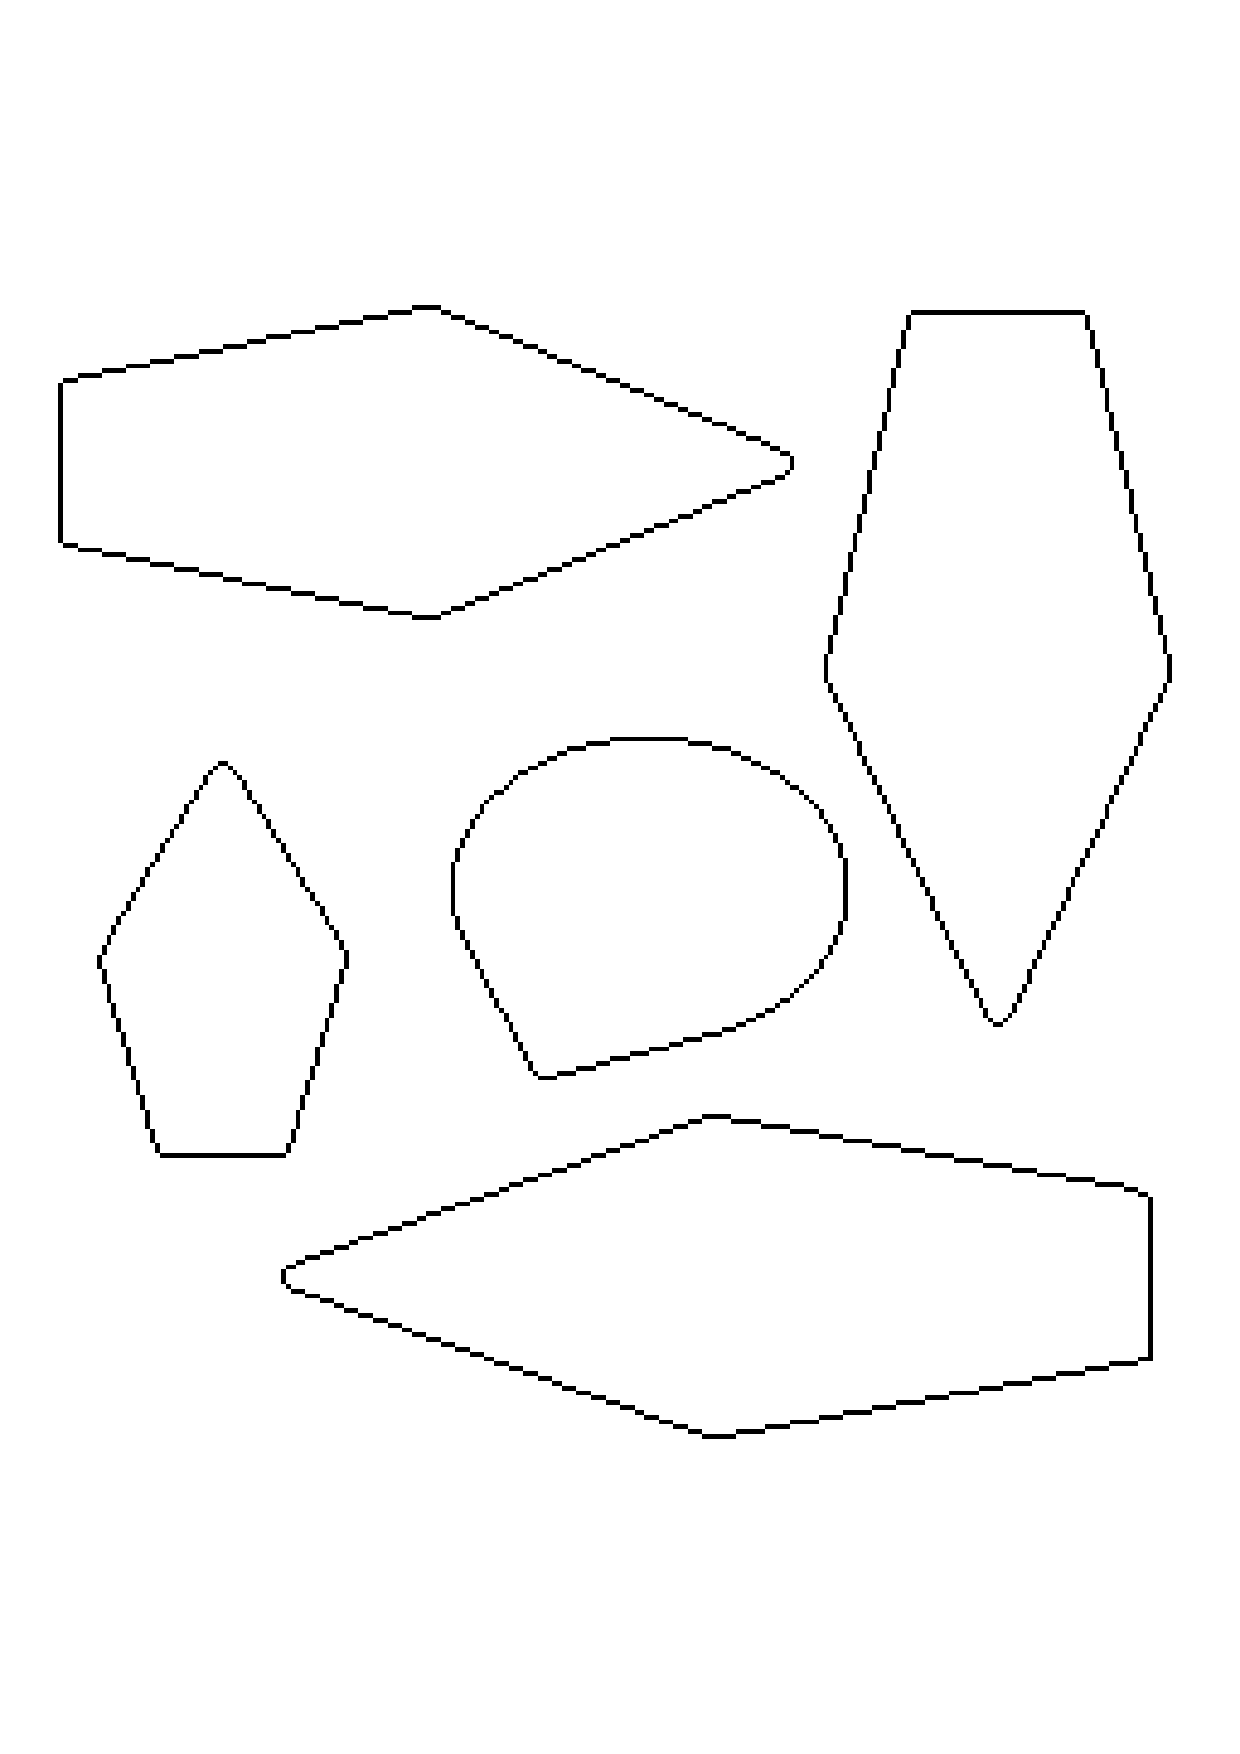
\includegraphics[scale=1]{./eremina_img/seq256.pdf}}
\caption{Последовательная реализация 256x256}
\end{figure}

\begin{figure}[H]
\center{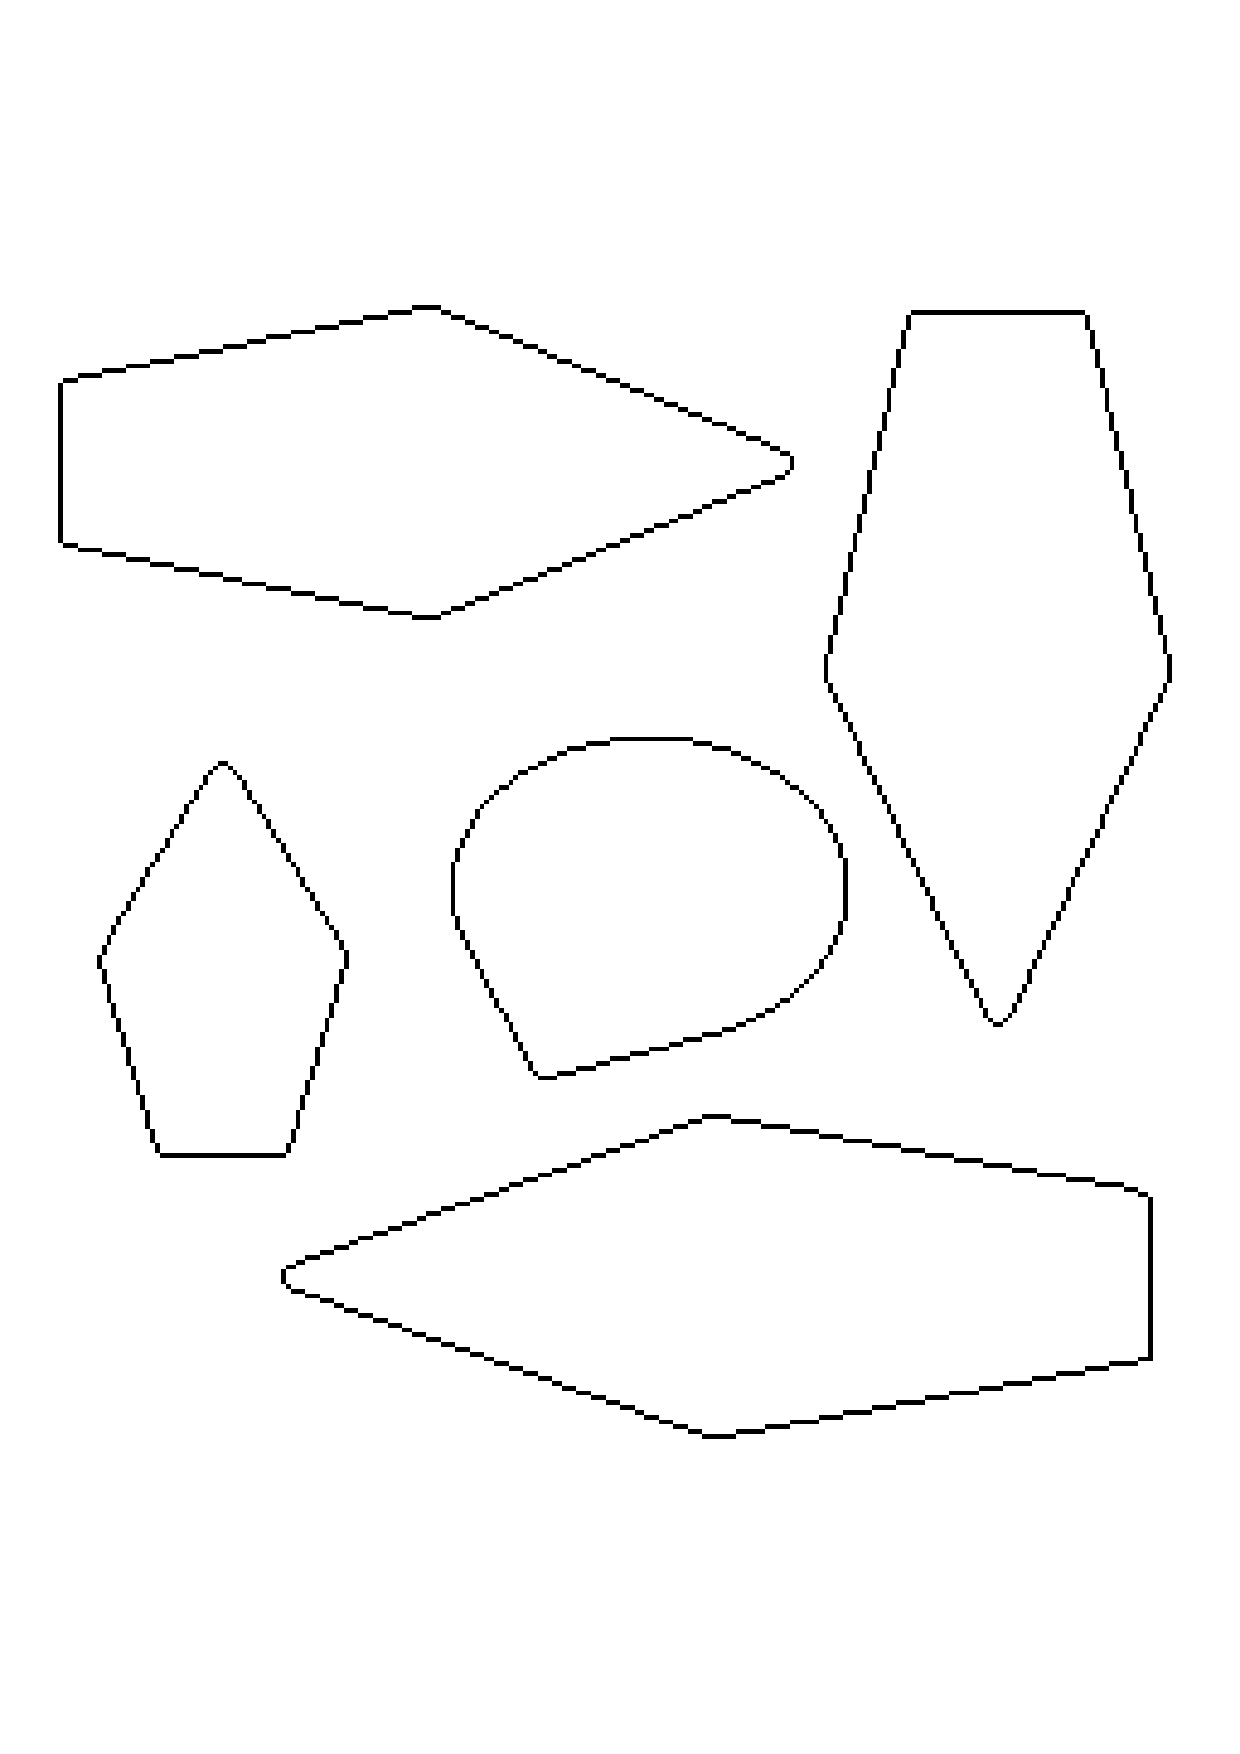
\includegraphics[scale=1]{./eremina_img/omp256.pdf}}
\caption{OMP реализация 256x256}
\end{figure}

\begin{figure}[H]
\center{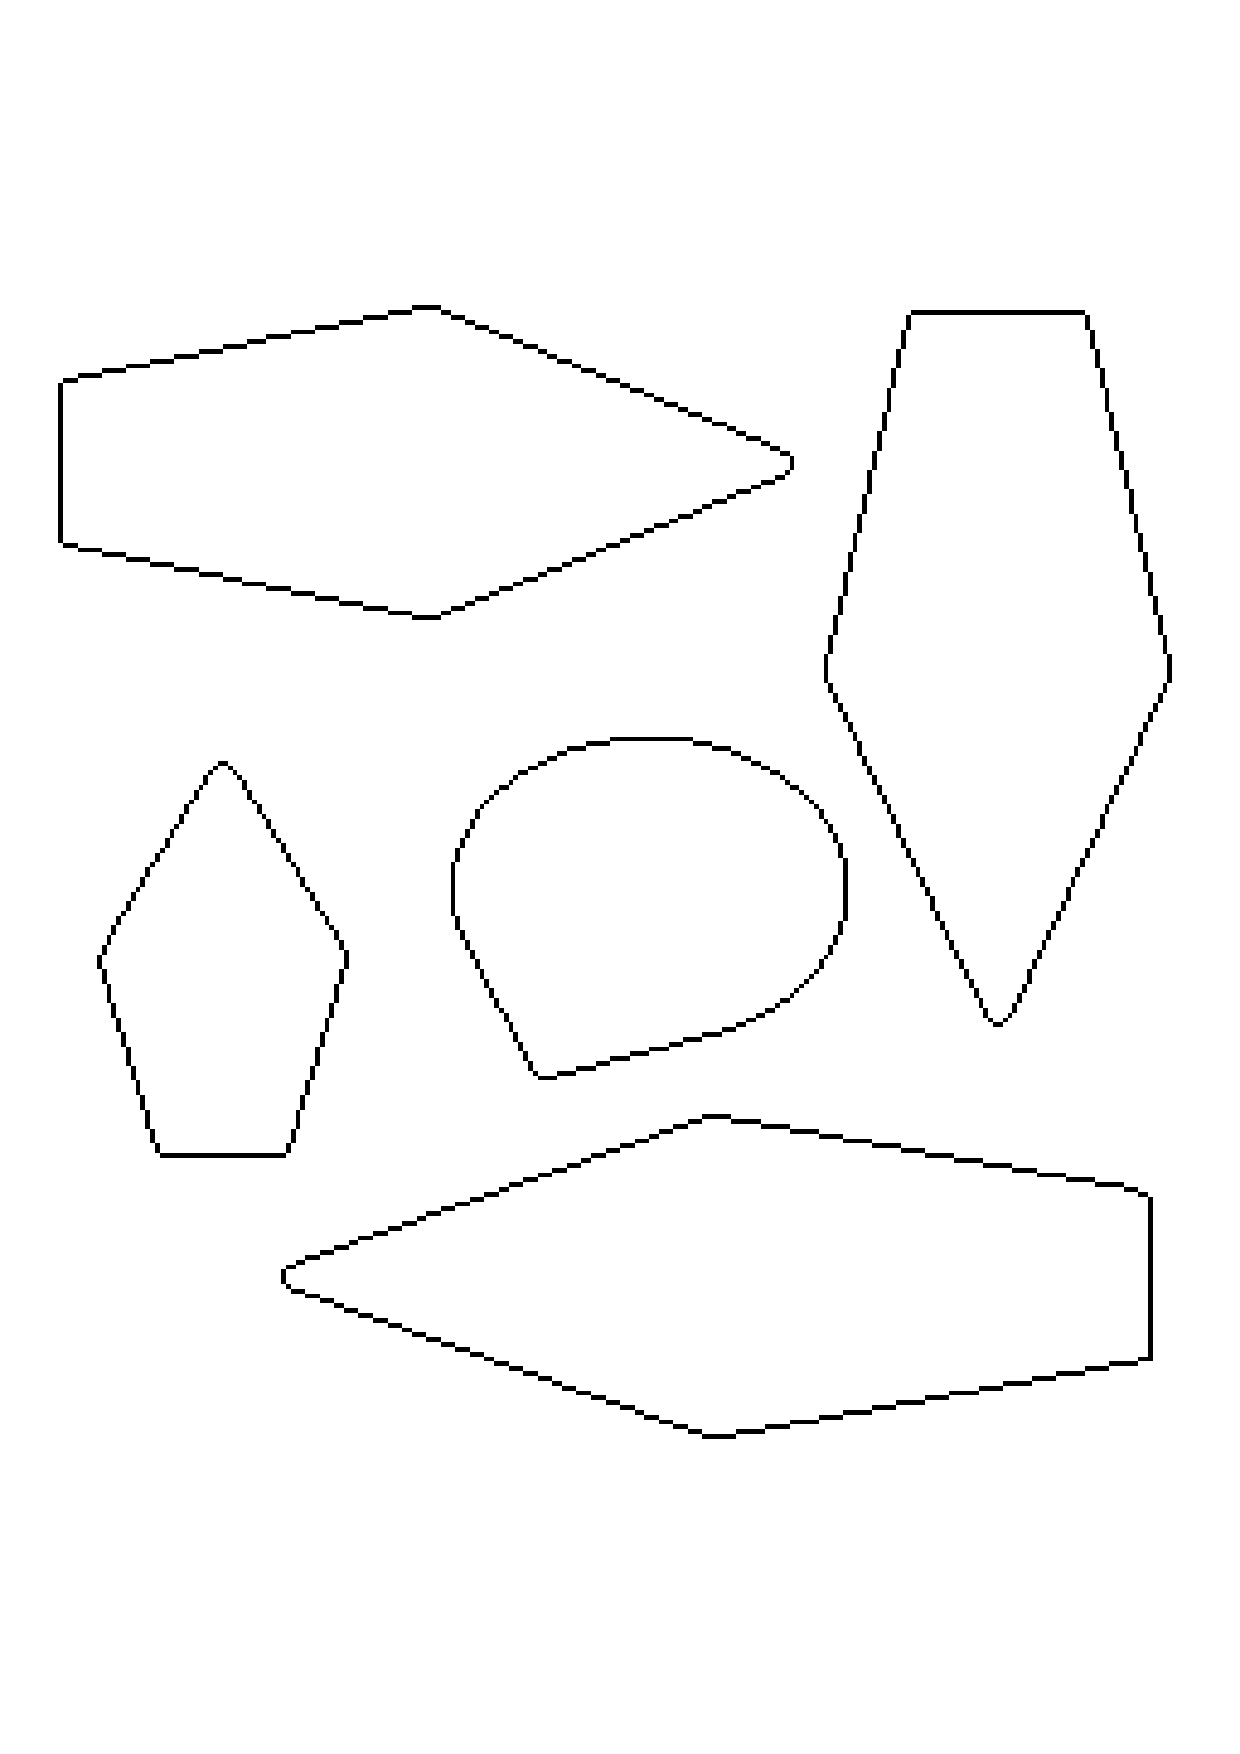
\includegraphics[scale=1]{./eremina_img/tbb256.pdf}}
\caption{TBB реализация 256x256}
\end{figure}

\begin{figure}[H]
\center{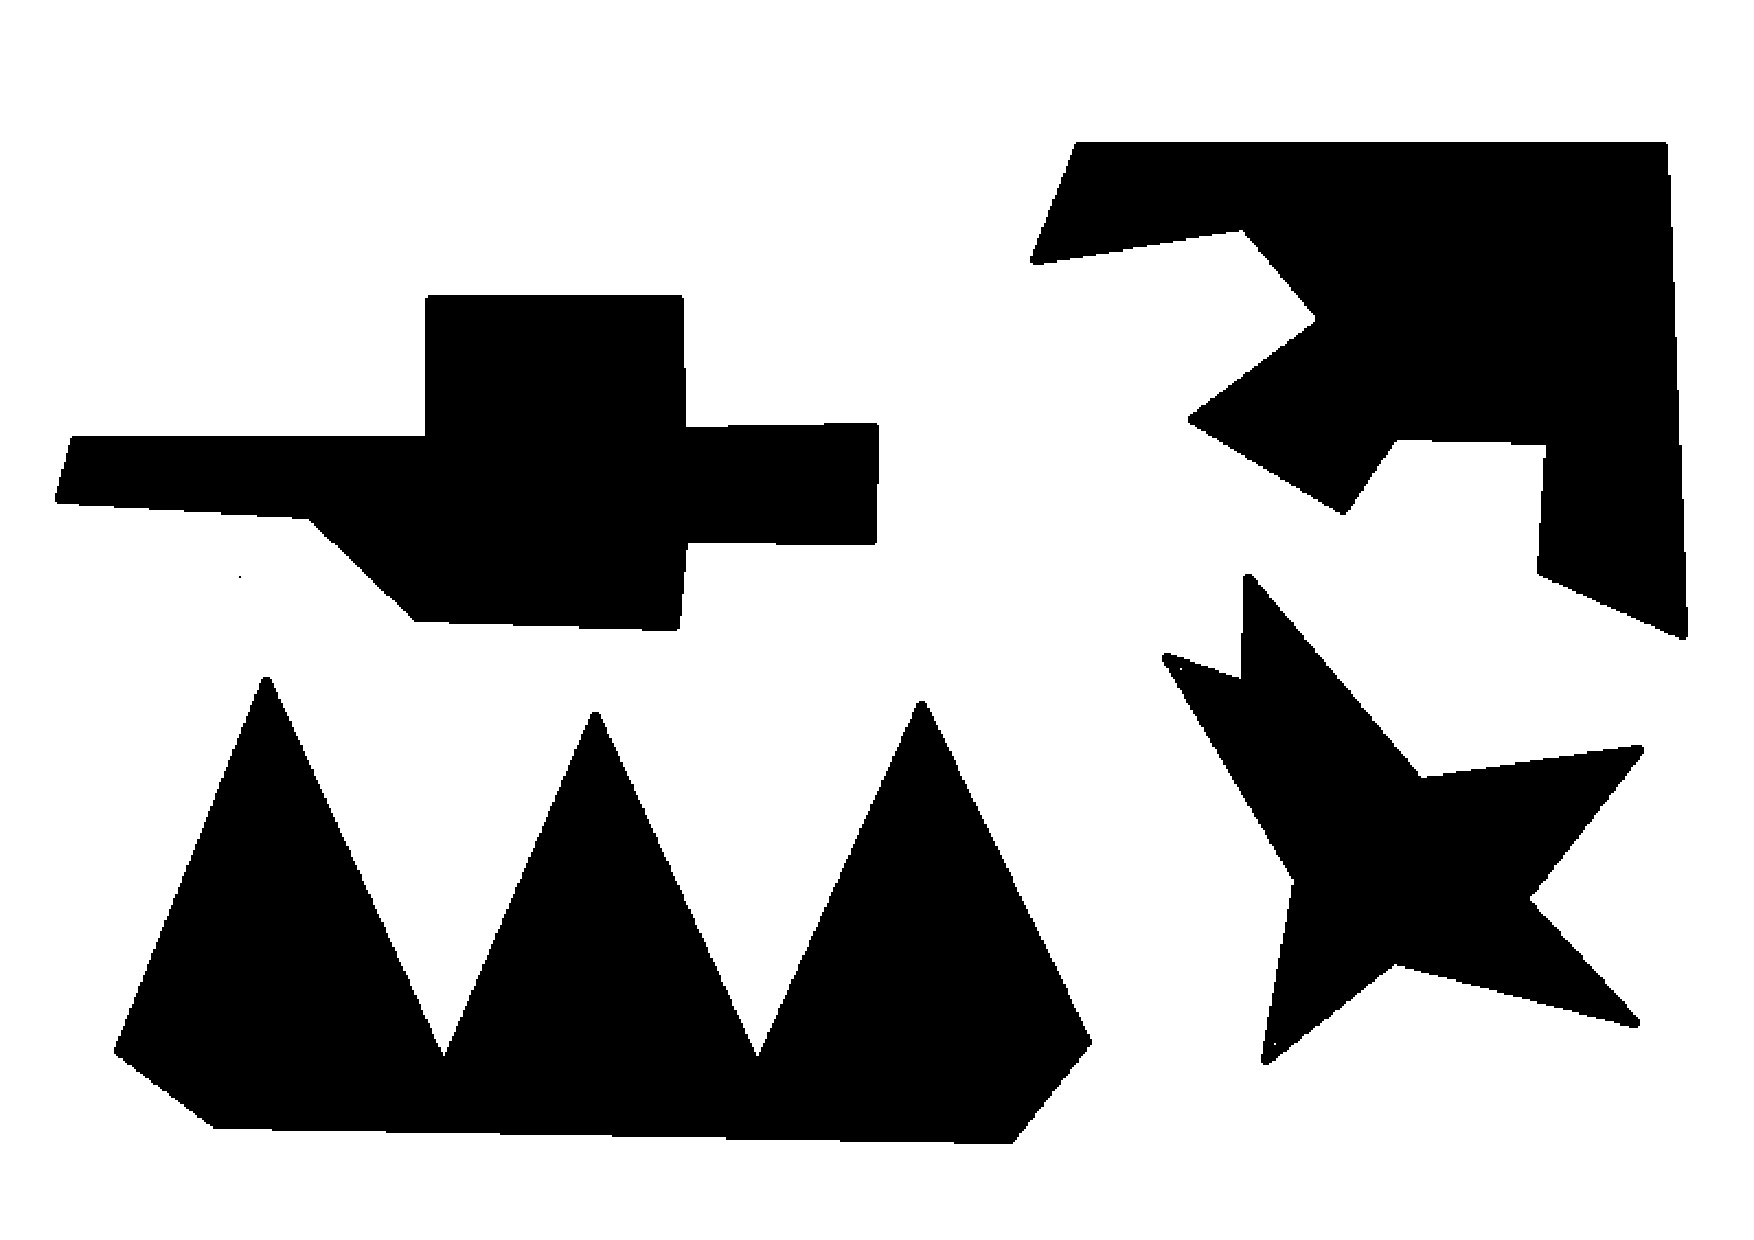
\includegraphics[scale=0.4]{./eremina_img/800x500.pdf}}
\caption{Бинарное изображение 800x500}
\end{figure}

\begin{figure}[H]
\center{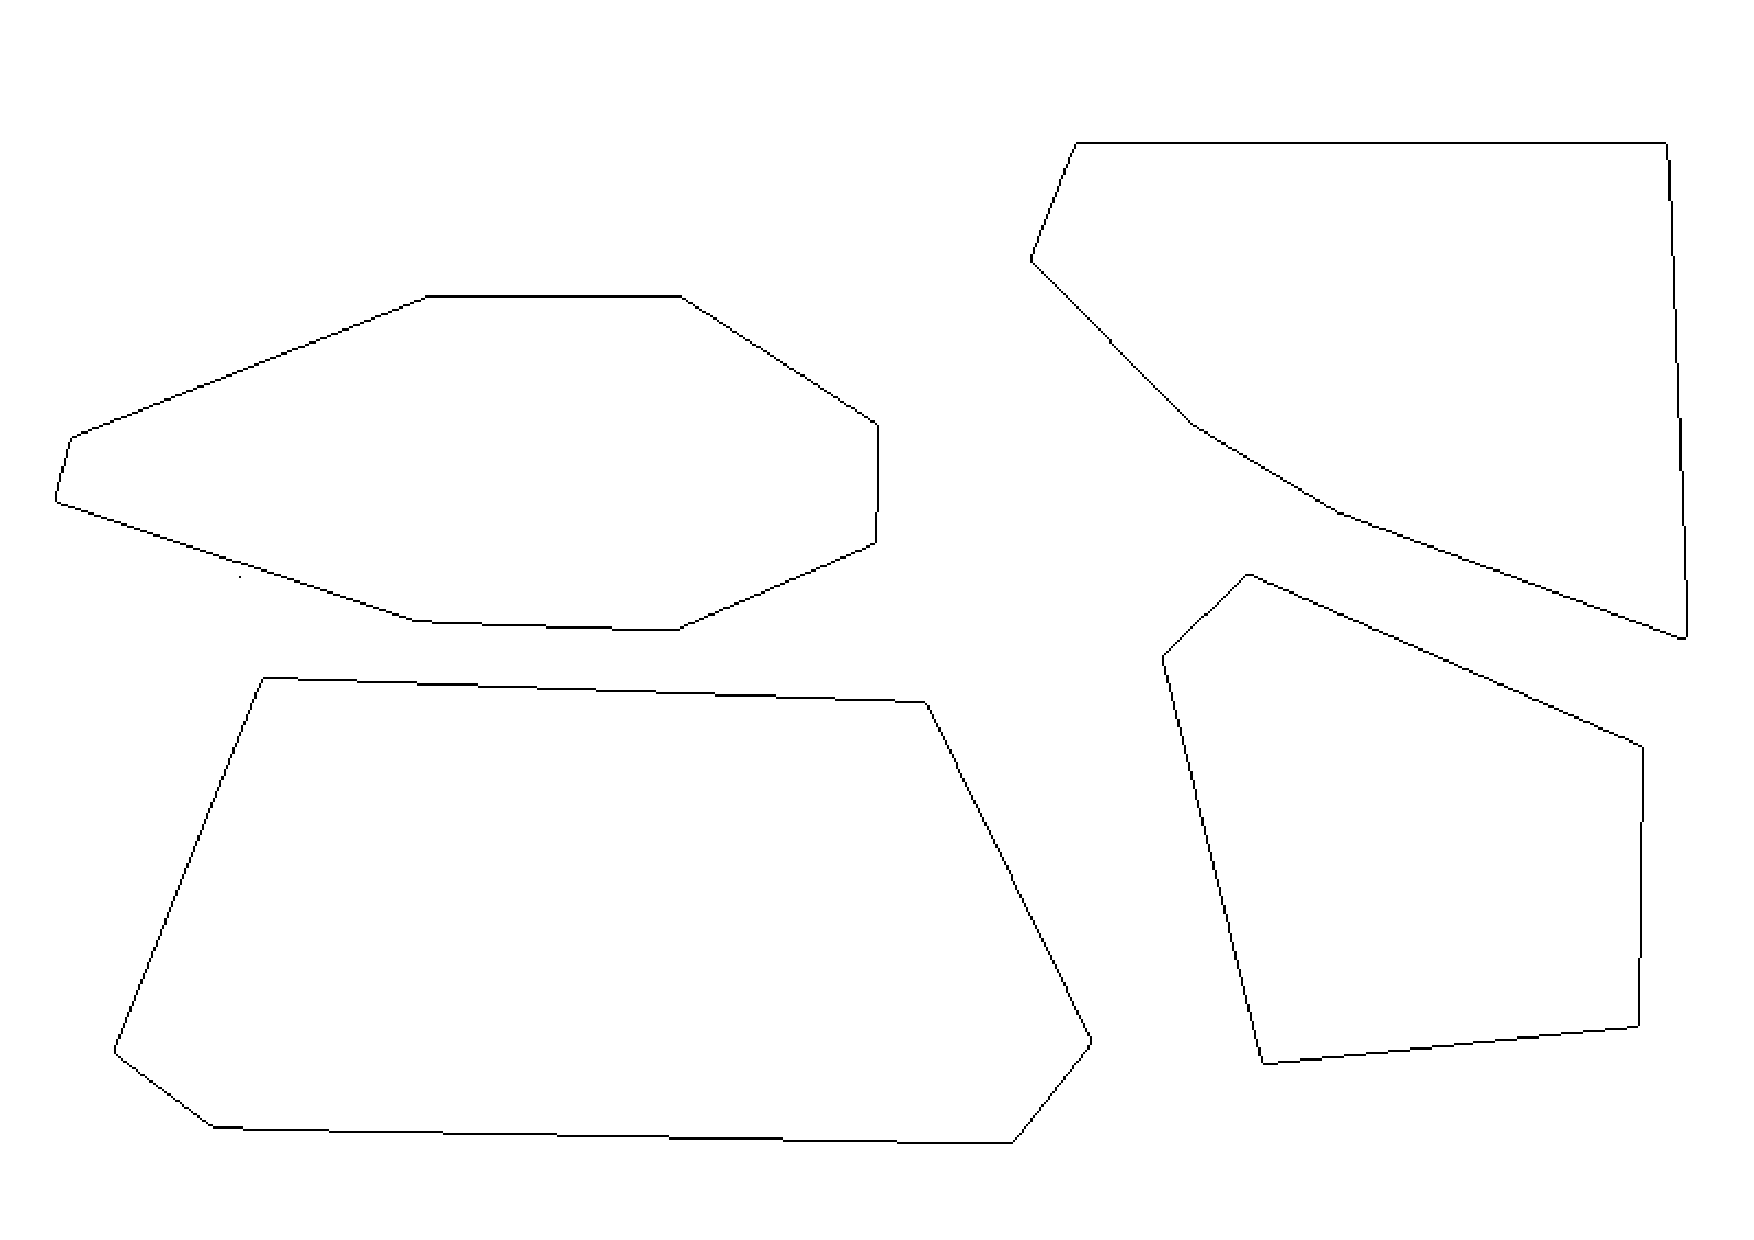
\includegraphics[scale=0.4]{./eremina_img/seq800x500.pdf}}
\caption{Последовательная реализация 800x500}
\end{figure}

\begin{figure}[H]
\center{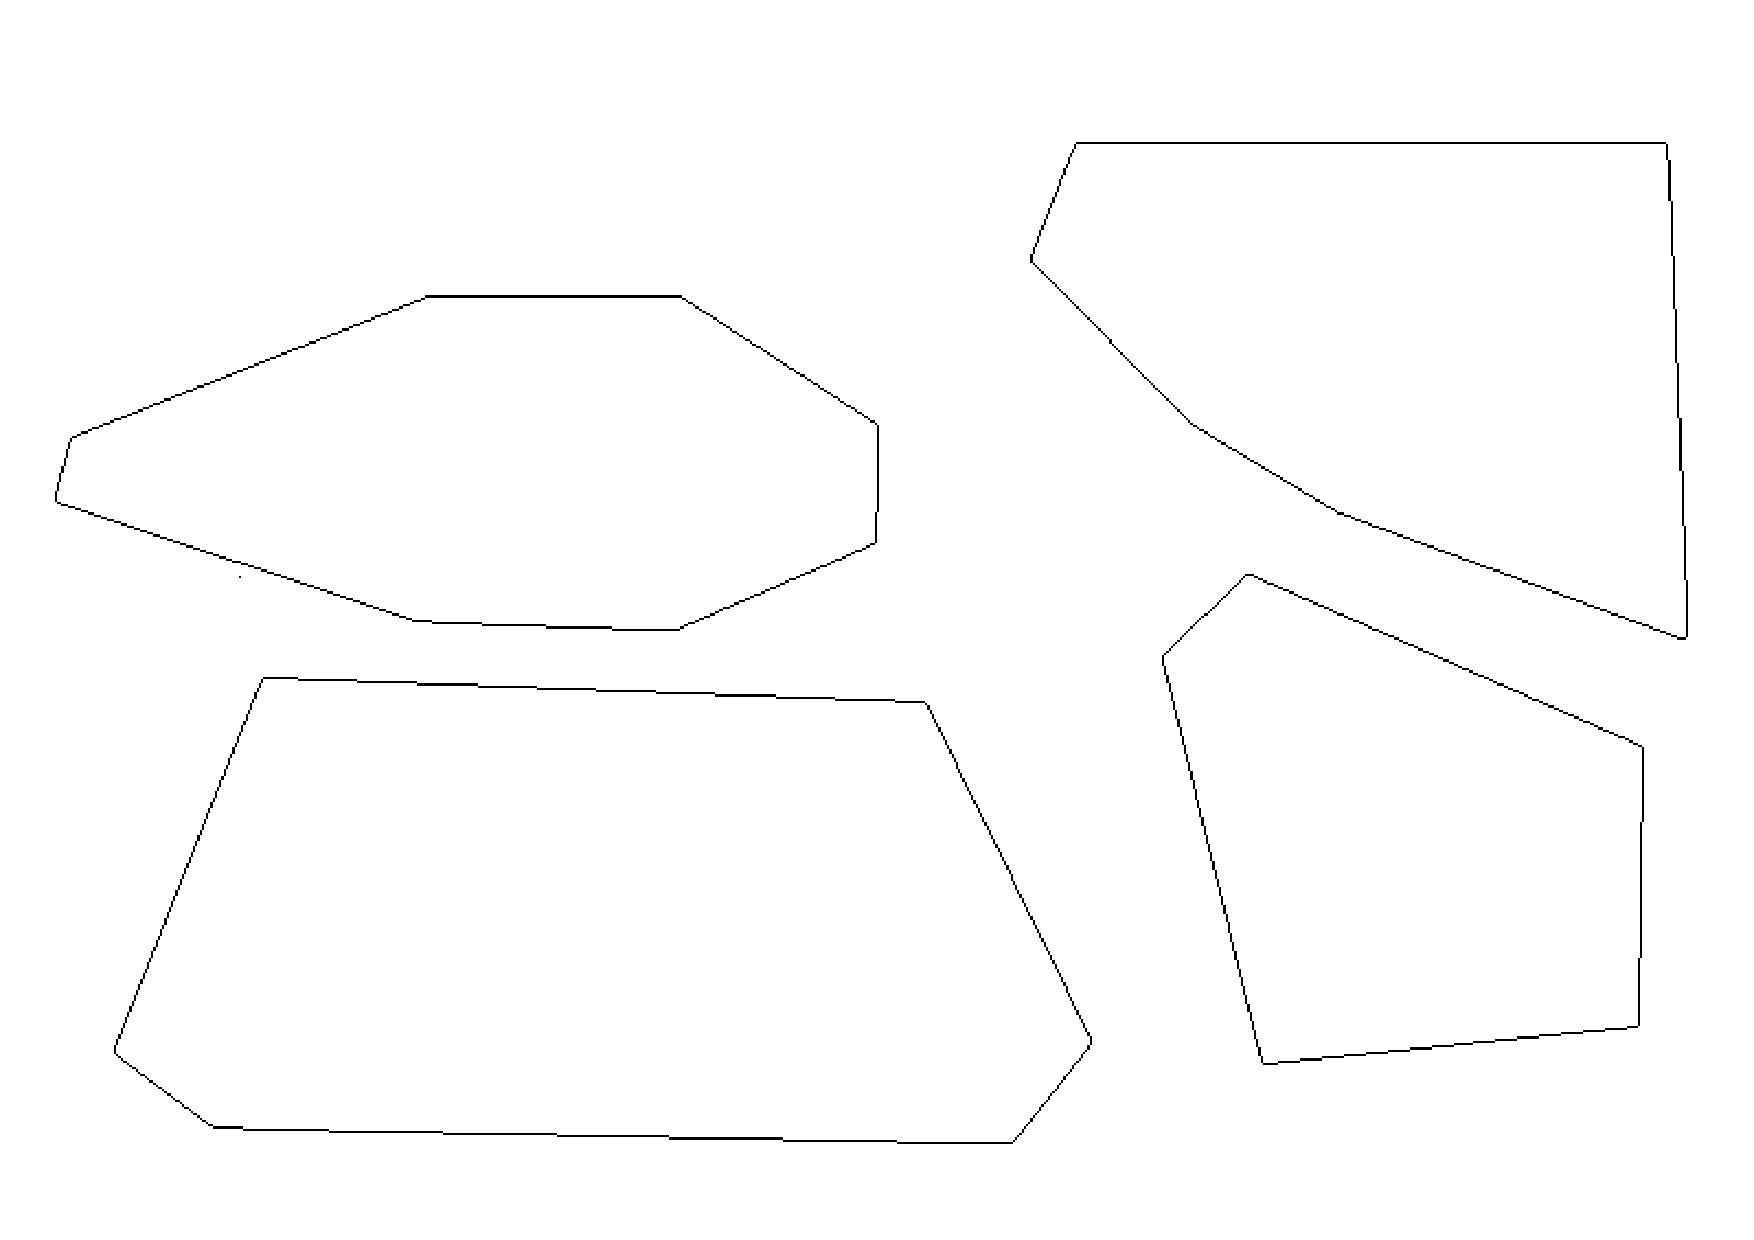
\includegraphics[scale=0.4]{./eremina_img/omp800x500.pdf}}
\caption{OMP реализация 800x500}
\end{figure}

\begin{figure}[H]
\center{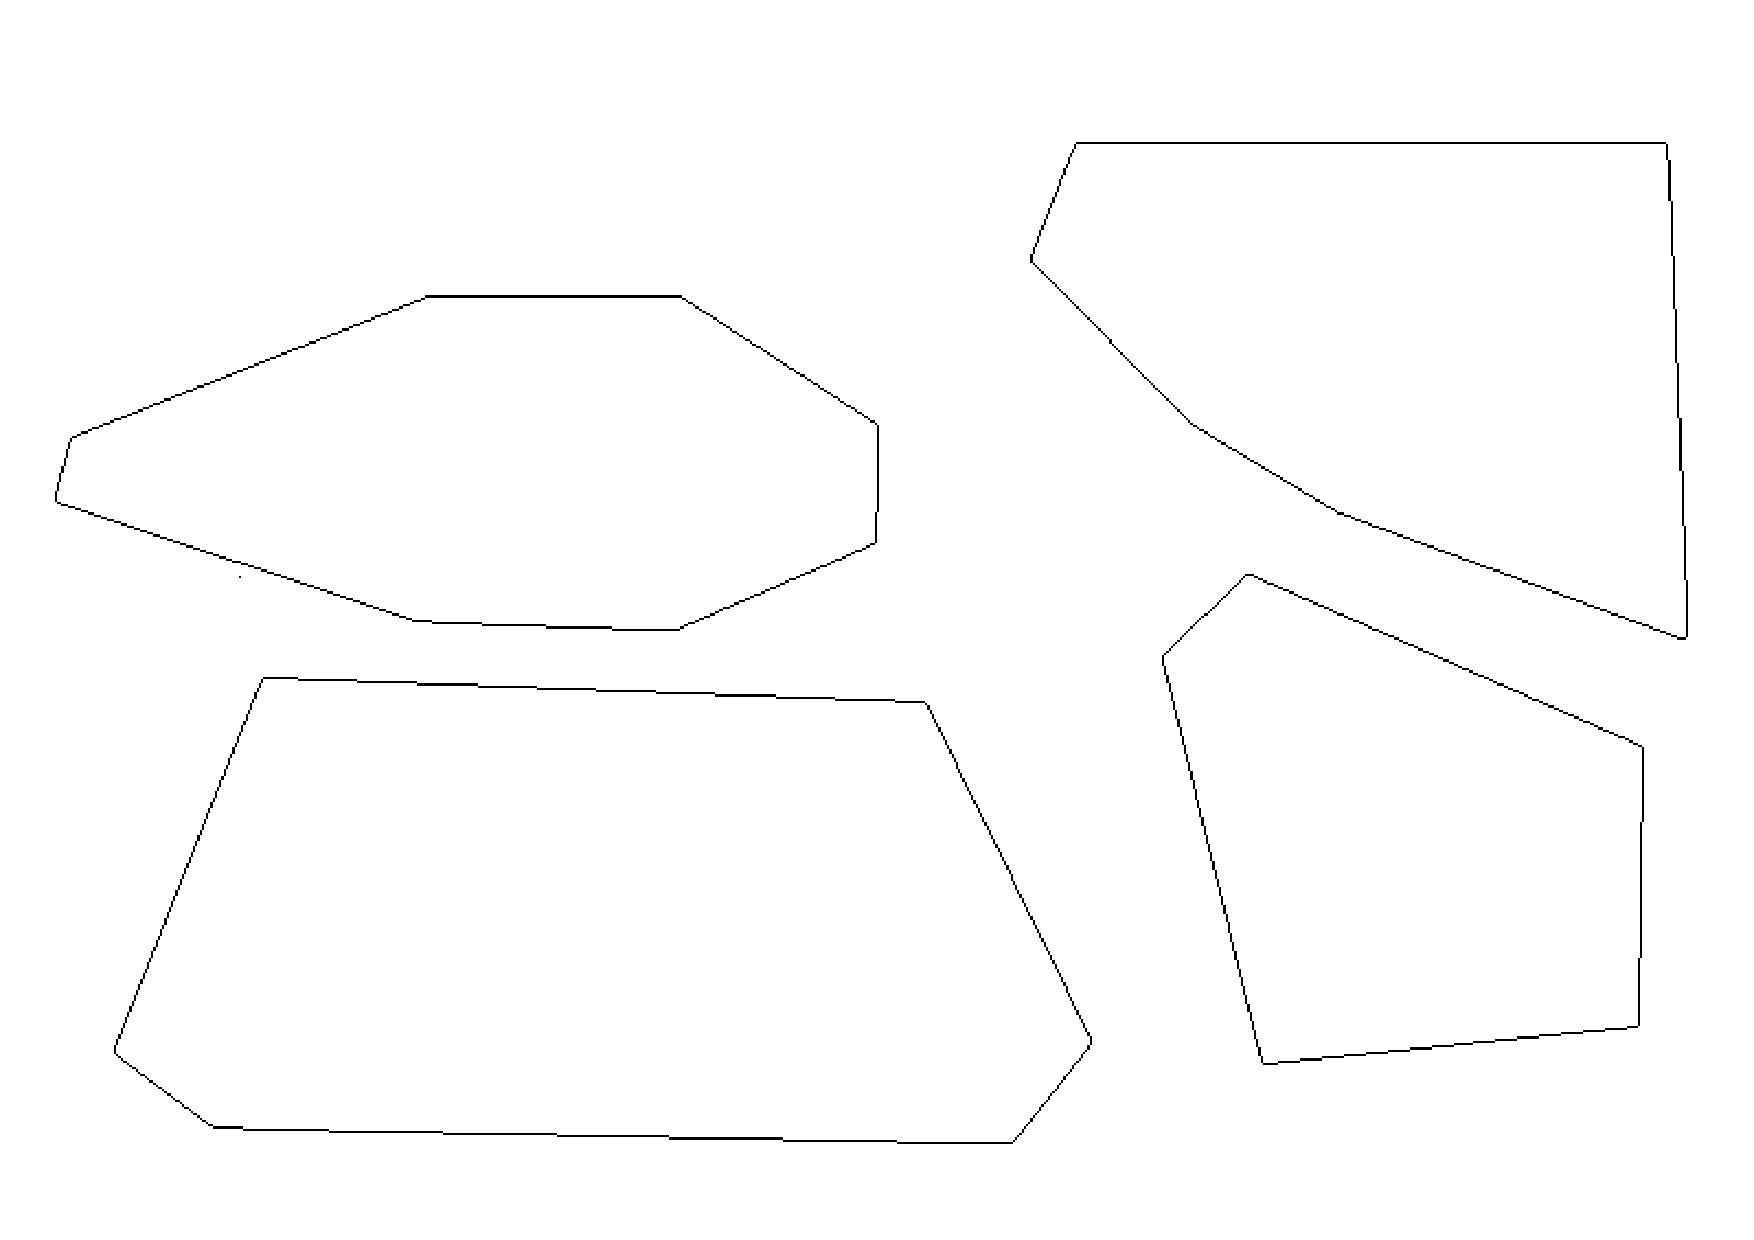
\includegraphics[scale=0.4]{./eremina_img/tbb800x500.pdf}}
\caption{TBB реализация 800x500}
\end{figure}

\begin{figure}[H]
\center{
\includegraphics[scale=0.2]{./eremina_img/1450x1000.pdf}}
\caption{Бинарное изображение 1450x1000}
\end{figure}

\begin{figure}[H]
\center{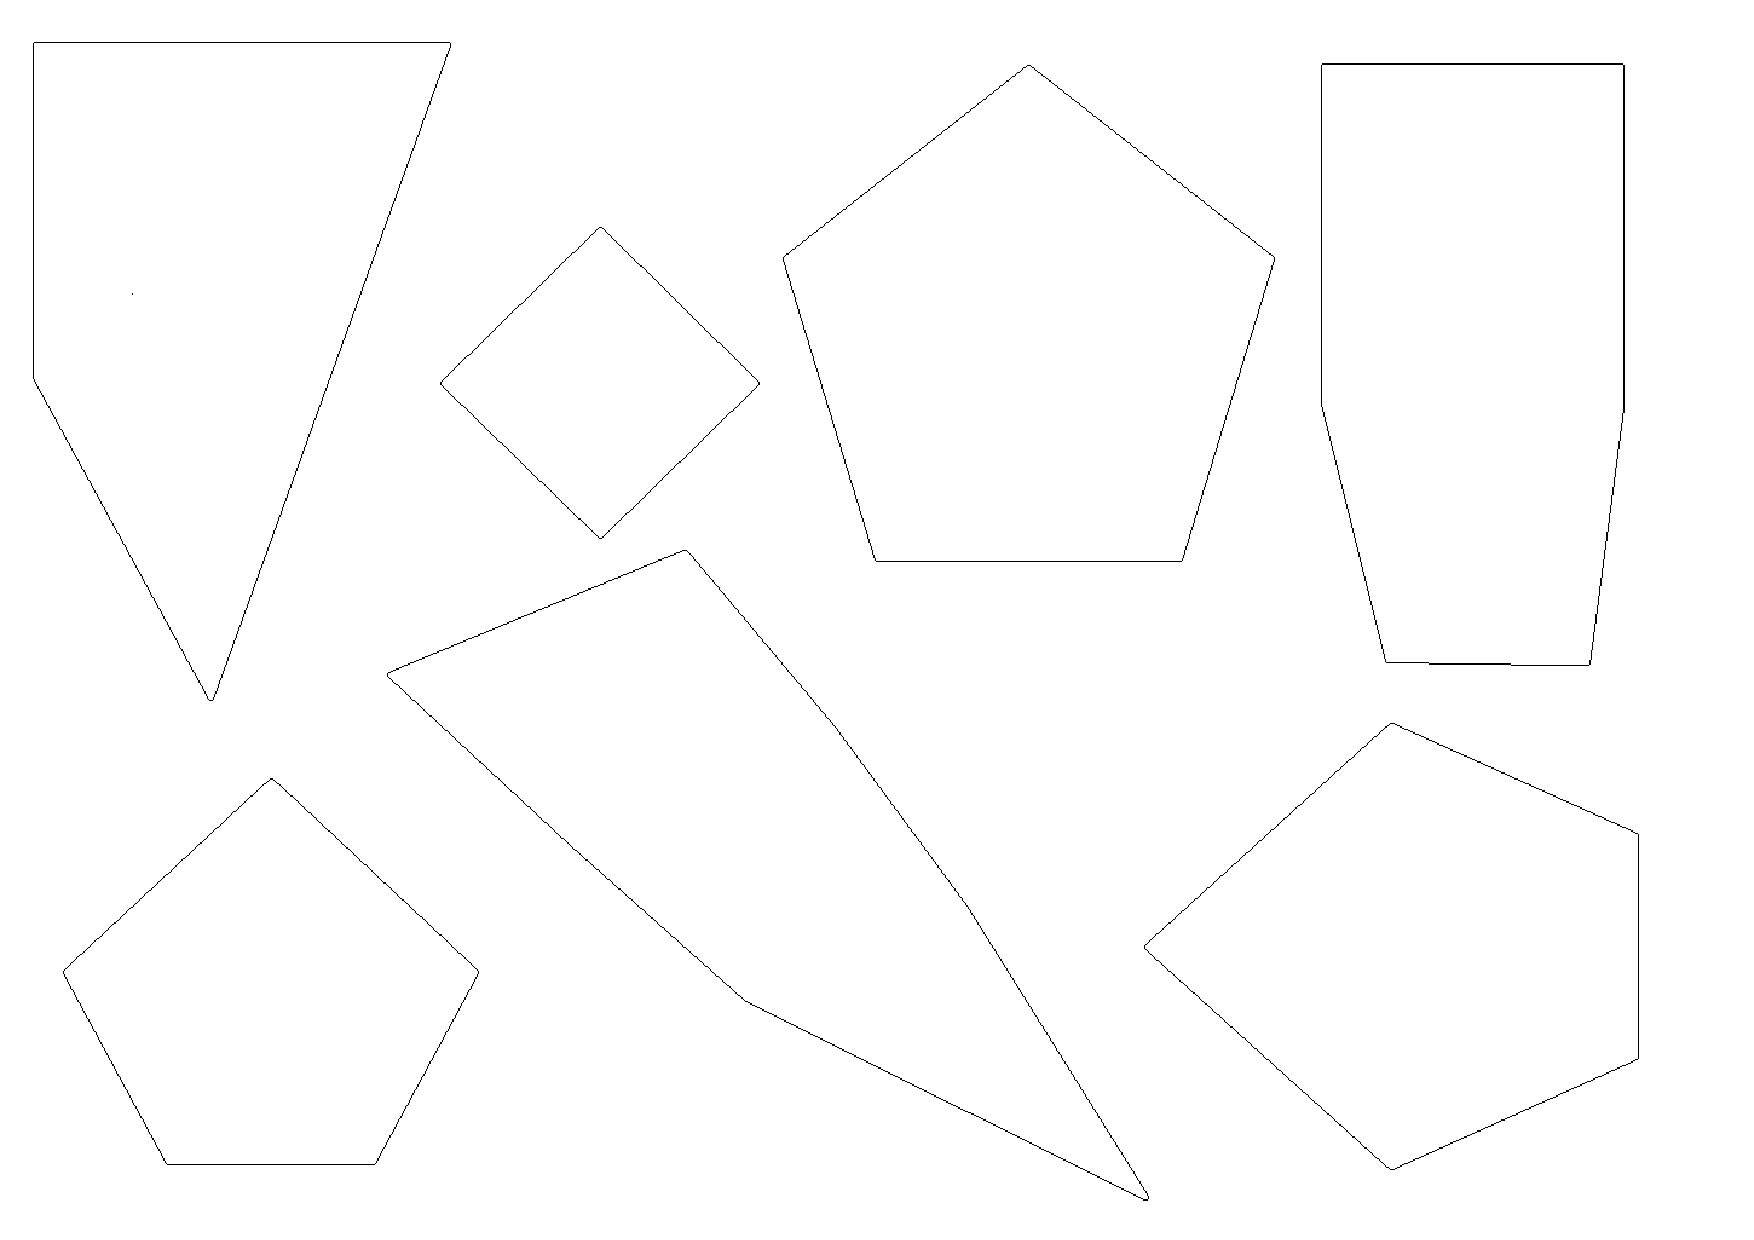
\includegraphics[scale=0.2]{./eremina_img/seq1450x1000.pdf}}
\caption{Последовательная реализация 1450x1000}
\end{figure}

\begin{figure}[H]
\center{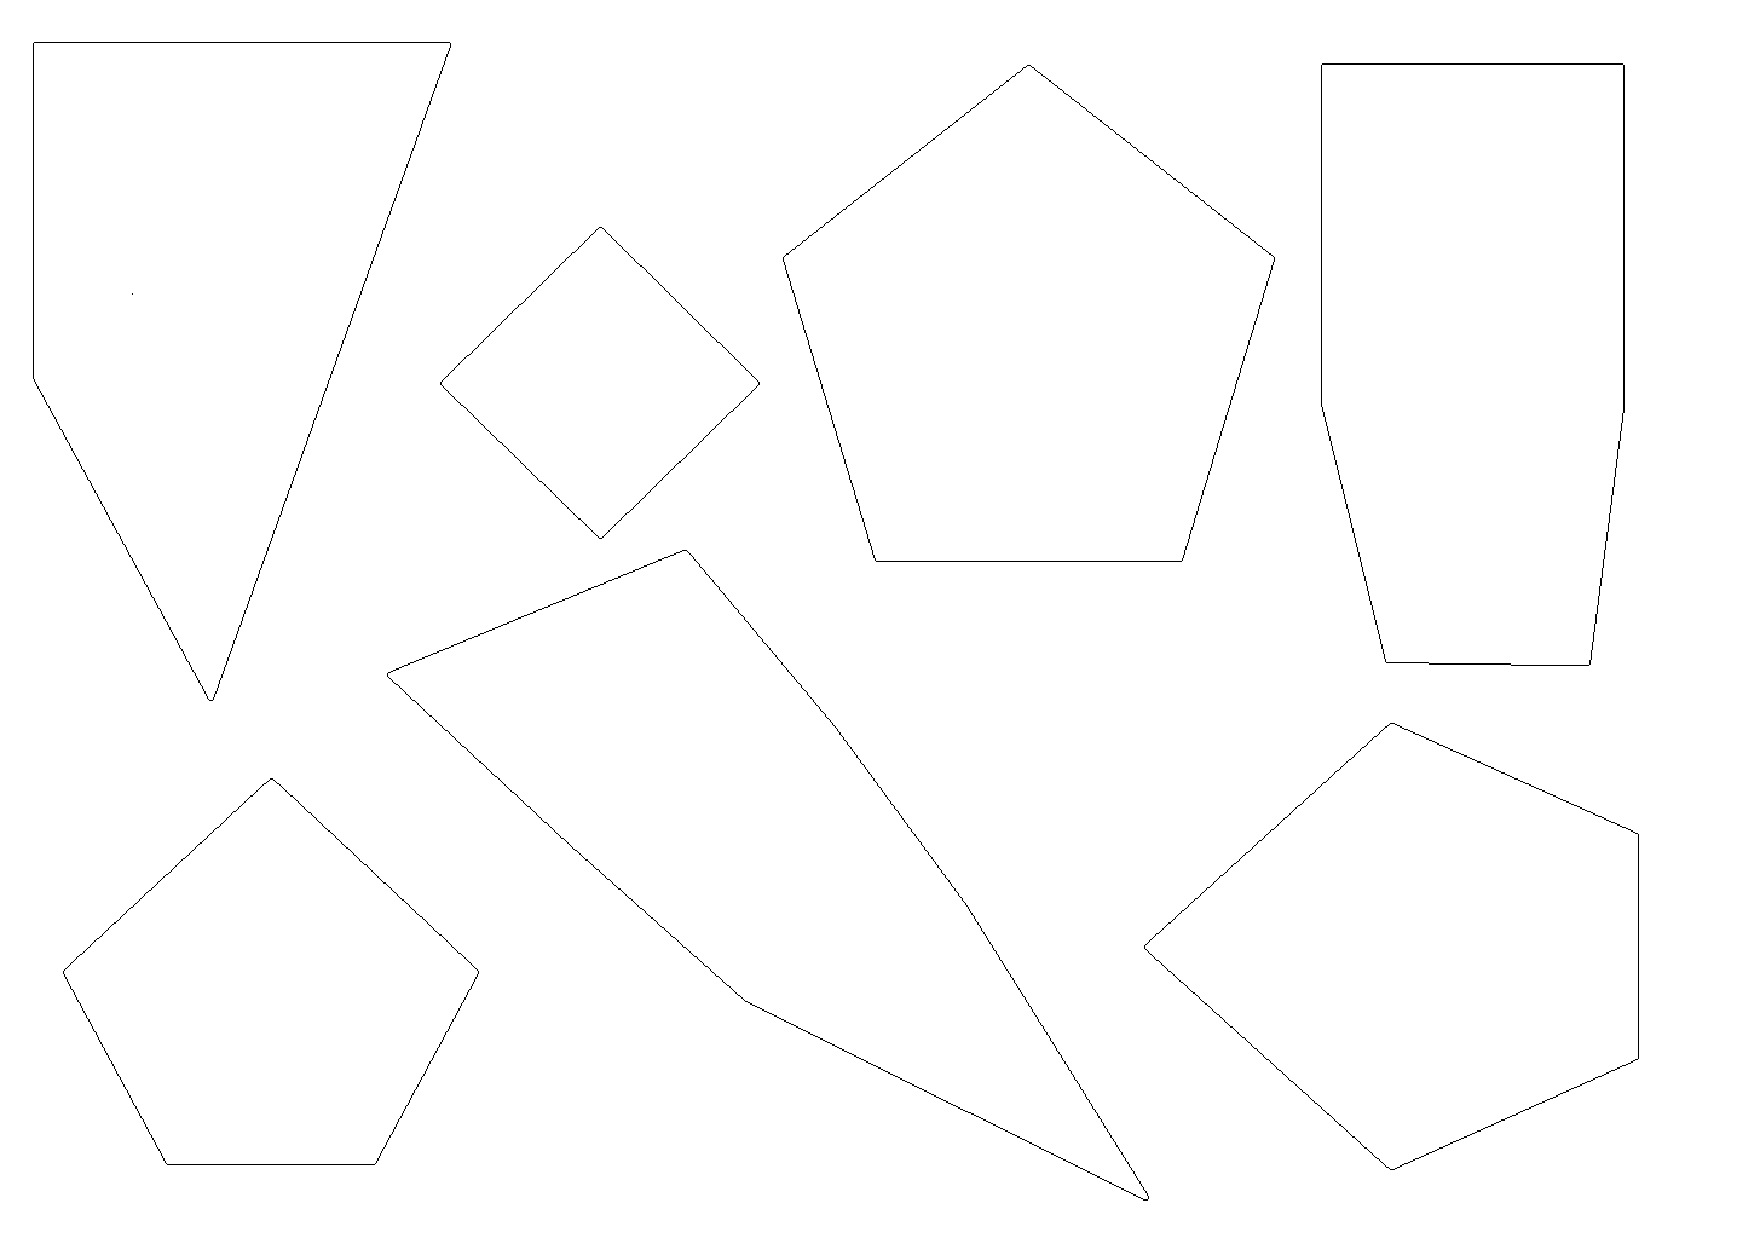
\includegraphics[scale=0.2]{./eremina_img/omp1450x1000.pdf}}
\caption{OMP реализация 1450x1000}
\end{figure}

\begin{figure}[H]
\center{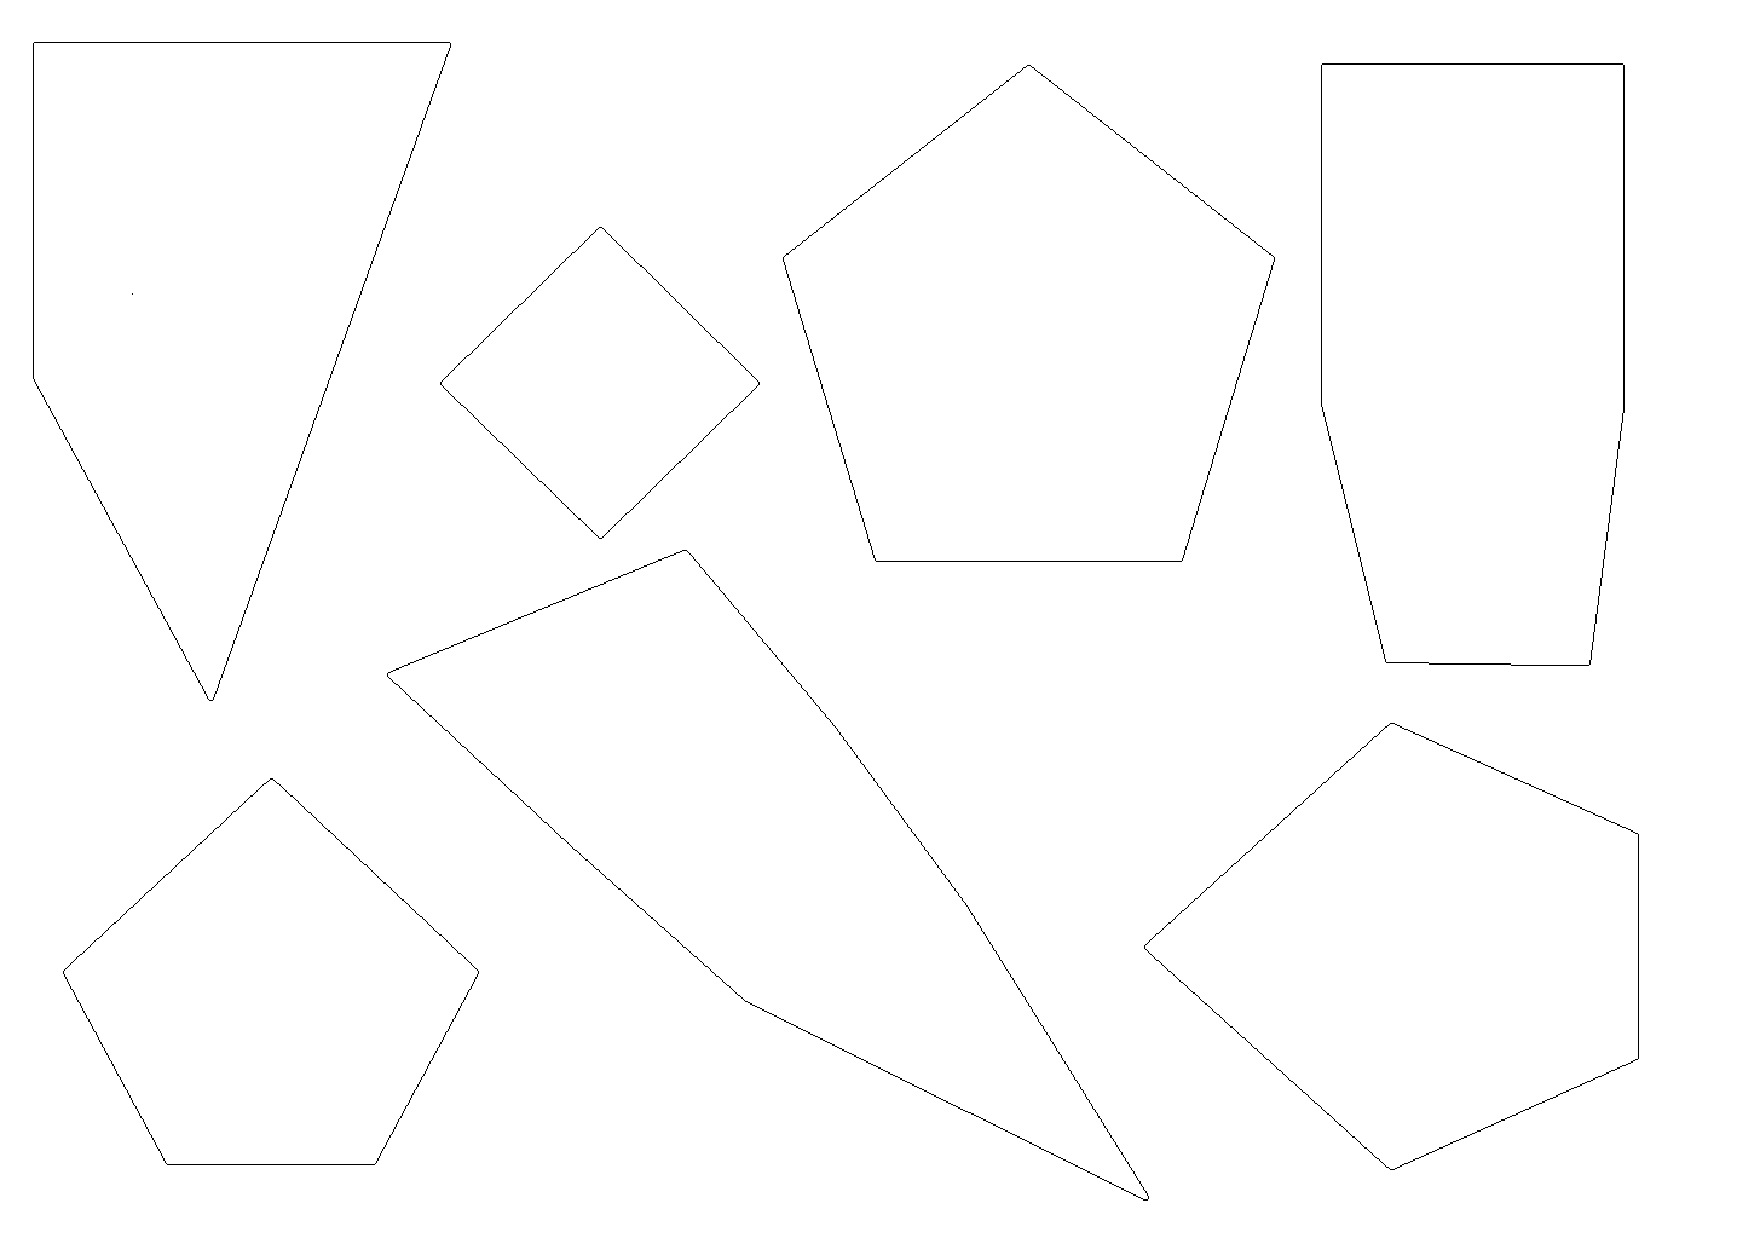
\includegraphics[scale=0.2]{./eremina_img/tbb1450x1000.pdf}}
\caption{TBB реализация 1450x1000}
\end{figure}

\par
Качественный анализ даёт понять, что алгоритмы работают корректно.

\newpage

% Заключение
\section*{Заключение}
\addcontentsline{toc}{section}{Заключение}
В ходе выполнения работы был успешно реализован алгоритм построения выпоклой оболочки для компонент бинарного изображения.
\par 
Основной задачей лабораторной работы была реализация эффективной параллельной версии. Эта цель была успешно достигнута, что подтверждается результатами экспериментов, проведенных в ходе работы. 
\par 
Работоспособность программы была проверена с помощью библиотеки для модульного тестирования, а также сравнительного анализа результирующих изображений.
\newpage

% Список литературы
\begin{thebibliography}{1}
\addcontentsline{toc}{section}{Список литературы}
\bibitem{Gergel}
Гергель В. П., Стронгин Р. Г. Основы параллельных вычислений для многопроцессорных вычислительных систем. – 2003.
\bibitem{Graham}
Алгоритм Грэхема: \url {https://en.wikipedia.org/wiki/Graham_scan }
\end{thebibliography}
\newpage

% Приложение
\section*{Приложение}
\addcontentsline{toc}{section}{Приложение}
\begin{lstlisting}
							// main.cpp

// Copyright 2021 Eremina Alena
#include <gtest/gtest.h>
#include <ctime>
#include "./convex_hull_bin.h"

TEST(Convex_Hull_Bin, Test_Convex_Bin_Random_Image_No_Throw) {
    int height = 20;
    int width = 40;
    std::vector<uint8_t> img_src(height * width);
    std::vector<uint8_t> img_dst(height * width, 255);
    img_src = generateImage(width, height);
    ASSERT_NO_THROW(img_dst = Convex_Hull(img_src, height, width));
}

TEST(Convex_Hull_Bin, Test_OMP_Convex_Bin_Random_Image_No_Throw) {
    int height = 20;
    int width = 40;
    std::vector<uint8_t> img_src(height * width);
    std::vector<uint8_t> img_dst(height * width, 255);
    img_src = generateImage(width, height);
    ASSERT_NO_THROW(img_dst = Convex_Hull_OMP(img_src, height, width));
}

TEST(Convex_Hull_Bin, Test_TBB_Convex_Bin_Random_Image_No_Throw) {
    int height = 20;
    int width = 40;
    std::vector<uint8_t> img_src(height * width);
    std::vector<uint8_t> img_dst(height * width, 255);
    img_src = generateImage(width, height);
    ASSERT_NO_THROW(img_dst = Convex_Hull_TBB(img_src, height, width));
}

TEST(Convex_Hull_Bin, Test_OMP_Convex_Bin_Random_Image) {
    int height = 20;
    int width = 40;
    std::vector<uint8_t> img_src(height * width);
    std::vector<uint8_t> img_dst_seq(height * width, 255);
    std::vector<uint8_t> img_dst_tbb(height * width, 255);
    img_src = generateImage(width, height);
    img_dst_seq = Convex_Hull(img_src, height, width);
    img_dst_tbb = Convex_Hull_OMP(img_src, height, width);
    int count = 0;
    for (int i = 0; i < height; i++) {
        for (int j = 0; j < width; j++) {
            if (img_dst_seq[i * width + j] == img_dst_tbb[i * width + j]) {
                count++;
            }
        }
    }
    double ratio = static_cast<double>(count)/(width*height);
    ASSERT_TRUE(ratio >= 0.95);
}
TEST(Convex_Hull_Bin, Test_TBB_Convex_Bin_Random_Image) {
    int height = 20;
    int width = 40;
    std::vector<uint8_t> img_src(height * width);
    std::vector<uint8_t> img_dst_seq(height * width, 255);
    std::vector<uint8_t> img_dst_tbb(height * width, 255);
    img_src = generateImage(width, height);
    img_dst_seq = Convex_Hull(img_src, height, width);
    img_dst_tbb = Convex_Hull_TBB(img_src, height, width);
    int count = 0;
    for (int i = 0; i < height; i++) {
        for (int j = 0; j < width; j++) {
            if (img_dst_seq[i * width + j] == img_dst_tbb[i * width + j]) {
                count++;
            }
        }
    }
    double ratio = static_cast<double>(count)/(width*height);
    ASSERT_TRUE(ratio >= 0.95);
}

TEST(Convex_Hull_Bin, Test_OMP_Convex_Bin_Small_Image) {
    int height = 8;
    int width = 8;
    std::vector<uint8_t> img_src = { 255, 255, 255, 255, 255, 255, 255, 255,
                                     255, 255, 255,   0, 255, 255, 255, 255,
                                     255, 255, 255,   0, 255, 255, 255, 255,
                                     255, 255, 255,   0,   0, 255, 255, 255,
                                     255, 255,   0,   0,   0,   0, 255, 255,
                                     255,   0,   0,   0,   0,   0,   0, 255,
                                     255, 255,   0,   0,   0,   0, 255, 255,
                                     255, 255, 255, 255, 255, 255, 255, 255 };
    std::vector<uint8_t> img_dst_seq(height * width);
    std::vector<uint8_t> img_dst_tbb(height * width);
    img_dst_seq = Convex_Hull(img_src, height, width);
    img_dst_tbb = Convex_Hull_OMP(img_src, height, width);
    int count = 0;
    for (int i = 0; i < height; i++) {
        for (int j = 0; j < width; j++) {
            if (img_dst_seq[i * width + j] == img_dst_tbb[i * width + j]) {
                count++;
            }
        }
    }
    double ratio = static_cast<double>(count)/(width*height);
    ASSERT_TRUE(ratio >= 0.95);
}

TEST(Convex_Hull_Bin, Test_TBB_Convex_Bin_Small_Image) {
    int height = 8;
    int width = 8;
    std::vector<uint8_t> img_src = { 255, 255, 255, 255, 255, 255, 255, 255,
                                     255, 255, 255,   0, 255, 255, 255, 255,
                                     255, 255, 255,   0, 255, 255, 255, 255,
                                     255, 255, 255,   0,   0, 255, 255, 255,
                                     255, 255,   0,   0,   0,   0, 255, 255,
                                     255,   0,   0,   0,   0,   0,   0, 255,
                                     255, 255,   0,   0,   0,   0, 255, 255,
                                     255, 255, 255, 255, 255, 255, 255, 255 };
    std::vector<uint8_t> img_dst_seq(height * width);
    std::vector<uint8_t> img_dst_tbb(height * width);
    img_dst_seq = Convex_Hull(img_src, height, width);
    img_dst_tbb = Convex_Hull_TBB(img_src, height, width);
    int count = 0;
    for (int i = 0; i < height; i++) {
        for (int j = 0; j < width; j++) {
            if (img_dst_seq[i * width + j] == img_dst_tbb[i * width + j]) {
                count++;
            }
        }
    }
    double ratio = static_cast<double>(count)/(width*height);
    ASSERT_TRUE(ratio >= 0.95);
}

TEST(Convex_Hull_Bin, Test_OMP_Convex_Bin_Medium_Image) {
    int height = 10;
    int width = 20;
    std::vector<uint8_t> img_src =
        { 255, 255, 255, 255,   0,   0, 255, 255, 255, 255,
          255, 255, 255, 255, 255, 255, 255, 255, 255, 255,
          255, 255, 255, 255,   0,   0, 255, 255, 255, 255,
          255,   0, 255, 255, 255, 255, 255, 255,   0, 255,
          255, 255, 255,   0,   0,   0, 255, 255, 255, 255,
          255, 255,   0, 255, 255, 255, 255,   0, 255, 255,
          255, 255, 255,   0,   0,   0, 255, 255, 255, 255,
          255, 255, 255,   0, 255, 255,   0, 255, 255, 255,
            0,   0,   0,   0,   0,   0,   0,   0,   0,   0,
          255, 255, 255, 255,   0,   0, 255, 255, 255, 255,
            0,   0,   0,   0,   0,   0,   0,   0, 255, 255,
          255, 255, 255, 255,   0,   0, 255, 255, 255, 255,
          255, 255, 255,   0,   0,   0,   0, 255, 255, 255,
          255, 255, 255,   0, 255, 255,   0, 255, 255, 255,
          255, 255, 255, 255,   0,   0,   0, 255, 255, 255,
          255, 255,   0, 255, 255, 255, 255,   0, 255, 255,
          255, 255, 255, 255,   0, 255, 255, 255, 255, 255,
          255,   0, 255, 255, 255, 255, 255, 255,   0, 255,
          255, 255, 255, 255,   0, 255, 255, 255, 255, 255,
          255, 255, 255, 255, 255, 255, 255, 255, 255, 255 };
    std::vector<uint8_t> img_dst_seq(height * width);
    std::vector<uint8_t> img_dst_tbb(height * width);
    img_dst_seq = Convex_Hull(img_src, height, width);
    img_dst_tbb = Convex_Hull_OMP(img_src, height, width);
    int count = 0;
    for (int i = 0; i < height; i++) {
        for (int j = 0; j < width; j++) {
            if (img_dst_seq[i * width + j] == img_dst_tbb[i * width + j]) {
                count++;
            }
        }
    }
    double ratio = static_cast<double>(count)/(width*height);
    ASSERT_TRUE(ratio >= 0.95);
}

TEST(Convex_Hull_Bin, Test_TBB_Convex_Bin_Medium_Image) {
    int height = 10;
    int width = 20;
    std::vector<uint8_t> img_src =
        { 255, 255, 255, 255,   0,   0, 255, 255, 255, 255,
          255, 255, 255, 255, 255, 255, 255, 255, 255, 255,
          255, 255, 255, 255,   0,   0, 255, 255, 255, 255,
          255,   0, 255, 255, 255, 255, 255, 255,   0, 255,
          255, 255, 255,   0,   0,   0, 255, 255, 255, 255,
          255, 255,   0, 255, 255, 255, 255,   0, 255, 255,
          255, 255, 255,   0,   0,   0, 255, 255, 255, 255,
          255, 255, 255,   0, 255, 255,   0, 255, 255, 255,
            0,   0,   0,   0,   0,   0,   0,   0,   0,   0,
          255, 255, 255, 255,   0,   0, 255, 255, 255, 255,
            0,   0,   0,   0,   0,   0,   0,   0, 255, 255,
          255, 255, 255, 255,   0,   0, 255, 255, 255, 255,
          255, 255, 255,   0,   0,   0,   0, 255, 255, 255,
          255, 255, 255,   0, 255, 255,   0, 255, 255, 255,
          255, 255, 255, 255,   0,   0,   0, 255, 255, 255,
          255, 255,   0, 255, 255, 255, 255,   0, 255, 255,
          255, 255, 255, 255,   0, 255, 255, 255, 255, 255,
          255,   0, 255, 255, 255, 255, 255, 255,   0, 255,
          255, 255, 255, 255,   0, 255, 255, 255, 255, 255,
          255, 255, 255, 255, 255, 255, 255, 255, 255, 255 };
    std::vector<uint8_t> img_dst_seq(height * width);
    std::vector<uint8_t> img_dst_tbb(height * width);
    img_dst_seq = Convex_Hull(img_src, height, width);
    img_dst_tbb = Convex_Hull_TBB(img_src, height, width);
    int count = 0;
    for (int i = 0; i < height; i++) {
        for (int j = 0; j < width; j++) {
            if (img_dst_seq[i * width + j] == img_dst_tbb[i * width + j]) {
                count++;
            }
        }
    }
    double ratio = static_cast<double>(count)/(width*height);
    ASSERT_TRUE(ratio >= 0.95);
}

TEST(Convex_Hull_Bin, Test_OMP_Convex_Bin_Large_Image) {
    int height = 32;
    int width = 20;
    std::vector<uint8_t> img_src =
    { 255, 255, 255, 255, 255, 255, 255, 255, 255, 255,
      255, 255, 255,   0,   0,   0,   0,   0,   0,   0,
      255, 255, 255, 255, 255, 255, 255, 255, 255, 255,
      255, 255, 255, 255, 255, 255, 255,   0,   0,   0,
      255, 255,   0,   0,   0,   0, 255, 255, 255, 255,
        0, 255, 255, 255, 255, 255, 255, 255,   0,   0,
      255, 255,   0,   0,   0,   0,   0,   0,   0, 255,
      255, 255, 255, 255, 255, 255, 255, 255, 255,   0,
      255,   0,   0,   0,   0,   0,   0,   0,   0, 255,
      255,   0, 255, 255, 255, 255, 255, 255, 255,   0,
      255,   0,   0,   0,   0,   0,   0,   0,   0, 255,
      255, 255, 255, 255, 255, 255, 255, 255, 255,   0,
      255,   0,   0,   0, 255, 255, 255, 255, 255, 255,
      255, 255, 255, 255, 255, 255, 255, 255, 255, 255,
      255,   0,   0,   0, 255, 255, 255, 255, 255, 255,
        0, 255, 255, 255, 255, 255, 255, 255, 255, 255,
      255,   0,   0,   0, 255, 255, 255, 255, 255, 255,
      255, 255, 255, 255, 255, 255, 255, 255, 255, 255,
      255,   0,   0, 255, 255, 255, 255, 255, 255, 255,
      255, 255, 255, 255, 255, 255, 255, 255, 255, 255,
      255,   0,   0, 255, 255, 255, 255, 255,   0,   0,
        0,   0,   0,   0,   0,   0,   0,   0, 255, 255,
      255, 255, 255, 255, 255, 255,   0,   0,   0,   0,
        0,   0,   0,   0,   0,   0,   0,   0,   0,   0,
      255, 255, 255, 255, 255, 255, 255, 255,   0,   0,
        0,   0,   0,   0,   0,   0,   0,   0, 255, 255,
      255, 255, 255, 255, 255, 255, 255, 255, 255, 255,
      255, 255, 255, 255, 255, 255, 255, 255, 255, 255,
      255, 255, 255, 255, 255, 255, 255, 255, 255, 255,
      255, 255, 255, 255, 255, 255, 255, 255, 255, 255,
      255, 255, 255, 255, 255, 255, 255, 255, 255, 255,
      255, 255, 255, 255, 255, 255, 255, 255, 255, 255,
      255, 255, 255, 255, 255, 255, 255, 255, 255, 255,
      255, 255, 255, 255, 255, 255, 255, 255, 255, 255,
      255, 255, 255, 255, 255, 255, 255, 255, 255, 255,
      255, 255, 255, 255, 255, 255, 255, 255, 255, 255,
      255, 255,   0,   0,   0,   0,   0,   0, 255, 255,
      255, 255, 255, 255, 255, 255, 255, 255, 255, 255,
      255,   0,   0,   0,   0,   0,   0,   0, 255, 255,
      255, 255, 255, 255, 255, 255, 255, 255, 255, 255,
      255,   0,   0,   0,   0,   0,   0,   0, 255, 255,
      255, 255, 255, 255, 255, 255, 255, 255, 255, 255,
        0,   0,   0,   0,   0,   0,   0,   0, 255, 255,
      255, 255, 255, 255, 255, 255, 255, 255, 255,   0,
        0,   0,   0,   0,   0,   0,   0,   0, 255, 255,
      255, 255, 255, 255, 255,   0,   0, 255,   0,   0,
        0,   0,   0,   0,   0,   0,   0, 255, 255, 255,
      255, 255, 255, 255,   0,   0,   0, 255,   0, 255,
      255, 255, 255, 255, 255, 255, 255, 255, 255, 255,
      255, 255, 255,   0,   0, 255,   0,   0,   0, 255,
      255, 255, 255, 255, 255, 255, 255, 255, 255, 255,
      255, 255, 255,   0, 255, 255,   0,   0, 255, 255,
      255, 255, 255, 255, 255, 255, 255, 255, 255, 255,
      255, 255,   0,   0, 255, 255, 255, 255, 255, 255,
      255, 255, 255, 255, 255, 255, 255, 255, 255, 255,
      255,   0,   0, 255, 255, 255, 255, 255, 255, 255,
      255, 255, 255, 255, 255, 255, 255, 255, 255, 255,
      255, 255, 255, 255, 255, 255, 255, 255, 255, 255,
      255, 255, 255, 255, 255, 255, 255, 255, 255, 255,
      255, 255, 255, 255, 255, 255, 255, 255, 255, 255,
      255, 255, 255, 255, 255, 255, 255, 255, 255, 255,
      255, 255, 255, 255, 255, 255, 255, 255, 255, 255,
      255, 255, 255, 255, 255, 255, 255, 255, 255, 255,
      255, 255, 255, 255, 255, 255, 255, 255, 255, 255 };

    std::vector<uint8_t> img_dst_seq(height * width);
    std::vector<uint8_t> img_dst_tbb(height * width);
    img_dst_seq = Convex_Hull(img_src, height, width);
    img_dst_tbb = Convex_Hull_OMP(img_src, height, width);
    int count = 0;
    for (int i = 0; i < height; i++) {
        for (int j = 0; j < width; j++) {
            if (img_dst_seq[i * width + j] == img_dst_tbb[i * width + j]) {
                count++;
            }
        }
    }
    double ratio = static_cast<double>(count)/(width*height);
    ASSERT_TRUE(ratio >= 0.95);
}

TEST(Convex_Hull_Bin, Test_TBB_Convex_Bin_Large_Image) {
    int height = 32;
    int width = 20;
    std::vector<uint8_t> img_src =
    { 255, 255, 255, 255, 255, 255, 255, 255, 255, 255,
      255, 255, 255,   0,   0,   0,   0,   0,   0,   0,
      255, 255, 255, 255, 255, 255, 255, 255, 255, 255,
      255, 255, 255, 255, 255, 255, 255,   0,   0,   0,
      255, 255,   0,   0,   0,   0, 255, 255, 255, 255,
        0, 255, 255, 255, 255, 255, 255, 255,   0,   0,
      255, 255,   0,   0,   0,   0,   0,   0,   0, 255,
      255, 255, 255, 255, 255, 255, 255, 255, 255,   0,
      255,   0,   0,   0,   0,   0,   0,   0,   0, 255,
      255,   0, 255, 255, 255, 255, 255, 255, 255,   0,
      255,   0,   0,   0,   0,   0,   0,   0,   0, 255,
      255, 255, 255, 255, 255, 255, 255, 255, 255,   0,
      255,   0,   0,   0, 255, 255, 255, 255, 255, 255,
      255, 255, 255, 255, 255, 255, 255, 255, 255, 255,
      255,   0,   0,   0, 255, 255, 255, 255, 255, 255,
        0, 255, 255, 255, 255, 255, 255, 255, 255, 255,
      255,   0,   0,   0, 255, 255, 255, 255, 255, 255,
      255, 255, 255, 255, 255, 255, 255, 255, 255, 255,
      255,   0,   0, 255, 255, 255, 255, 255, 255, 255,
      255, 255, 255, 255, 255, 255, 255, 255, 255, 255,
      255,   0,   0, 255, 255, 255, 255, 255,   0,   0,
        0,   0,   0,   0,   0,   0,   0,   0, 255, 255,
      255, 255, 255, 255, 255, 255,   0,   0,   0,   0,
        0,   0,   0,   0,   0,   0,   0,   0,   0,   0,
      255, 255, 255, 255, 255, 255, 255, 255,   0,   0,
        0,   0,   0,   0,   0,   0,   0,   0, 255, 255,
      255, 255, 255, 255, 255, 255, 255, 255, 255, 255,
      255, 255, 255, 255, 255, 255, 255, 255, 255, 255,
      255, 255, 255, 255, 255, 255, 255, 255, 255, 255,
      255, 255, 255, 255, 255, 255, 255, 255, 255, 255,
      255, 255, 255, 255, 255, 255, 255, 255, 255, 255,
      255, 255, 255, 255, 255, 255, 255, 255, 255, 255,
      255, 255, 255, 255, 255, 255, 255, 255, 255, 255,
      255, 255, 255, 255, 255, 255, 255, 255, 255, 255,
      255, 255, 255, 255, 255, 255, 255, 255, 255, 255,
      255, 255, 255, 255, 255, 255, 255, 255, 255, 255,
      255, 255,   0,   0,   0,   0,   0,   0, 255, 255,
      255, 255, 255, 255, 255, 255, 255, 255, 255, 255,
      255,   0,   0,   0,   0,   0,   0,   0, 255, 255,
      255, 255, 255, 255, 255, 255, 255, 255, 255, 255,
      255,   0,   0,   0,   0,   0,   0,   0, 255, 255,
      255, 255, 255, 255, 255, 255, 255, 255, 255, 255,
        0,   0,   0,   0,   0,   0,   0,   0, 255, 255,
      255, 255, 255, 255, 255, 255, 255, 255, 255,   0,
        0,   0,   0,   0,   0,   0,   0,   0, 255, 255,
      255, 255, 255, 255, 255,   0,   0, 255,   0,   0,
        0,   0,   0,   0,   0,   0,   0, 255, 255, 255,
      255, 255, 255, 255,   0,   0,   0, 255,   0, 255,
      255, 255, 255, 255, 255, 255, 255, 255, 255, 255,
      255, 255, 255,   0,   0, 255,   0,   0,   0, 255,
      255, 255, 255, 255, 255, 255, 255, 255, 255, 255,
      255, 255, 255,   0, 255, 255,   0,   0, 255, 255,
      255, 255, 255, 255, 255, 255, 255, 255, 255, 255,
      255, 255,   0,   0, 255, 255, 255, 255, 255, 255,
      255, 255, 255, 255, 255, 255, 255, 255, 255, 255,
      255,   0,   0, 255, 255, 255, 255, 255, 255, 255,
      255, 255, 255, 255, 255, 255, 255, 255, 255, 255,
      255, 255, 255, 255, 255, 255, 255, 255, 255, 255,
      255, 255, 255, 255, 255, 255, 255, 255, 255, 255,
      255, 255, 255, 255, 255, 255, 255, 255, 255, 255,
      255, 255, 255, 255, 255, 255, 255, 255, 255, 255,
      255, 255, 255, 255, 255, 255, 255, 255, 255, 255,
      255, 255, 255, 255, 255, 255, 255, 255, 255, 255,
      255, 255, 255, 255, 255, 255, 255, 255, 255, 255 };

    std::vector<uint8_t> img_dst_seq(height * width);
    std::vector<uint8_t> img_dst_tbb(height * width);
    img_dst_seq = Convex_Hull(img_src, height, width);
    img_dst_tbb = Convex_Hull_TBB(img_src, height, width);
    int count = 0;
    for (int i = 0; i < height; i++) {
        for (int j = 0; j < width; j++) {
            if (img_dst_seq[i * width + j] == img_dst_tbb[i * width + j]) {
                count++;
            }
        }
    }
    double ratio = static_cast<double>(count)/(width*height);
    ASSERT_TRUE(ratio >= 0.95);
}

int main(int argc, char **argv) {
    ::testing::InitGoogleTest(&argc, argv);
    return RUN_ALL_TESTS();
}

\end{lstlisting}
\begin{lstlisting}
							// convex_hull_bin.cpp

// Copyright 2021 Eremina Alena
#include "../../../modules/task_3/eremina_a_convex_hull_bin/convex_hull_bin.h"

#include <tbb/blocked_range.h>
#include <tbb/mutex.h>
#include <tbb/parallel_for.h>
#include <tbb/task_scheduler_init.h>

#include <math.h>
#include <map>
#include <vector>
#include <stack>
#include <random>
#include <ctime>
#define PI 3.1416

int fun_min(int a, int b) {
    if (a > b) {
        return b;
    }
    return a;
}

int fun_max(int a, int b) {
    if (a > b) {
        return a;
    }
    return b;
}

// Generate binary image
std::vector<uint8_t> generateImage(const int wigth, const int height) {
    std::vector<uint8_t> img_src_dst(wigth*height);
    std::mt19937 gen;
    gen.seed(static_cast<unsigned int>(time(0)));
    for (int i = 0; i < wigth * height; i++) {
        int r = gen() % 5;
        if (r == 0) {
            img_src_dst[i] = 0;  // black
        } else {
            img_src_dst[i] = 255;  // white
        }
    }
    return img_src_dst;
}

// Split binary image into components
std::map<int, int> splitImageIntoComponents(std::vector<int>* img_src_dst,
    const int width, const int height) {
    int kn = 0, km = 0;
    int count = 1;
    int A, B, C;
    for (int i = 0; i < height; i++) {
        for (int j = 0; j < width; j++) {
            kn = j - 1;
            if (kn < 0) {
                kn = 0;
                B = 0;
            } else {
                B = img_src_dst->data()[i * width + kn];
            }
            km = i - 1;
            if (km < 0) {
                km = 0;
                C = 0;
            } else {
                C = img_src_dst->data()[km * width + j];
            }
            A = img_src_dst->data()[i * width + j];
            if (A == 0) {
                continue;
            } else if (B == 0 && C ==0) {
                count++;
                img_src_dst->data()[i * width + j] = count;
            } else if (B != 0 && C == 0) {
                img_src_dst->data()[i * width + j] = B;
            } else if (B == 0 && C != 0) {
                img_src_dst->data()[i * width + j] = C;
            } else if (B != 0 && C != 0) {
                if (B == C) {
                    img_src_dst->data()[i * width + j] = B;
                } else {
                    img_src_dst->data()[i * width + j] = B;
                    for (int u = 0; u < height; u++) {
                        for (int v = 0; v < width; v++) {
                            if (img_src_dst->data()[u * width + v] == C) {
                                img_src_dst->data()[u * width + v] = B;
                            }
                        }
                    }
                }
            }
        }
    }

    std::map<int, int> marks;
    for (int i = 0; i < height; i++) {
        for (int j = 0; j < width; j++) {
            if (img_src_dst->data()[i * width + j] == 0) {
                continue;
            } else {
                auto f = marks.find(img_src_dst->data()[i * width + j]);
                if (f != marks.end()) {
                    int count = f->second + 1;
                    marks[img_src_dst->data()[i * width + j]] = count;
                } else {
                    marks[img_src_dst->data()[i * width + j]] = 1;
                }
            }
        }
    }

    return marks;
}

// Sort points in ascending order of polar angle,
// measured counterclockwise from point p0;
// If the polar angles of several points coincide,
// then the distance to the point p0
void sortPolar(point* points, const point* p0, const int count) {
    for (int i = 0; i < count; i++) {
        int y = points[i].y - p0->y;
        int x = points[i].x - p0->x;
        double polar_angle = atan2(y, x);
        if (polar_angle < 0) polar_angle += 2*PI;
        points[i].polar_angle = polar_angle;
        points[i].distanse_p0 = sqrt(x * x + y * y);
    }

    point temp = {0, 0, 0, 0};
    for (int i = 0; i < count - 1; i++) {
        for (int j = 0; j < count - i - 1; j++) {
            if (points[j].polar_angle > points[j + 1].polar_angle) {
                temp = points[j];
                points[j] = points[j + 1];
                points[j + 1] = temp;
            } else if (abs(points[j].polar_angle - points[j + 1].polar_angle)
                       < 0.000001) {
                if (points[j].distanse_p0 < points[j + 1].distanse_p0
                    && points[j].distanse_p0 != 0) {
                    temp = points[j];
                    points[j] = points[j + 1];
                    points[j + 1] = temp;
                }
            }
        }
    }
}

// Do the three points a, b and c make a right turn (with or without =)?
bool rightTurn(const point* a, const point* b, const point* c, bool flag) {
    point u = {b->x - a->x, b->y - a->y, 0, 0};
    point v = {c->x - b->x, c->y - b->y, 0, 0};
    if (flag) {
        return u.x * v.y - u.y * v.x <= 0;
    }
    return u.x * v.y - u.y * v.x < 0;
}

// Graham's algorithm - an algorithm for constructing a convex hull
// in two-dimensional space
std::vector<uint8_t> Convex_Hull(std::vector<uint8_t> img_src,
    const int height, const int width) {
    // Output data
    std::vector<uint8_t> img_dst(height * width, 255);

    // Copy img_src to img_mark
    std::vector<int> img_mark(height * width);
    for (int i = 0; i < height; i++) {
        for (int j = 0; j < width; j++) {
            if (img_src[i * width + j] == 0) {
                img_mark[i * width + j] = 1;
            } else {
                img_mark[i * width + j] = 0;
            }
        }
    }

    // Split binary image into components
    std::map<int, int> marks = splitImageIntoComponents(&img_mark,
        width, height);

    for (auto mark : marks) {
        if (mark.second <= 3) {
            int cnt = 0;
            for (int i = 0; i < height && cnt < mark.second; i++) {
                for (int j = 0; j < width && cnt < mark.second; j++) {
                    if (img_mark[i * width + j] == mark.first) {
                        img_dst[i * width + j] = 0;
                        cnt++;
                    }
                }
            }
            continue;
        }
        // p0 - point with the minimum Y or the leftmost one
        point p0 = {width, height, 0, 0};
        // points - array of all points of the component
        point* points = new point[mark.second];
        // count - number of founded points of the component
        int count = 0;

        // find p0
        for (int i = 0; i < height && count < mark.second; i++) {
            for (int j = 0; j < width && count < mark.second; j++) {
                if (img_mark[i * width + j] == mark.first) {
                    points[count] = {j, i, 0, 0};
                    count++;
                    if (i < p0.y) {
                        p0.x = j;
                        p0.y = i;
                    }
                    if (i == p0.y) {
                        if (j < p0.x) {
                            p0.x = j;
                            p0.y = i;
                        }
                    }
                }
            }
        }

        // Sort points
        sortPolar(points, &p0, count);

        std::stack<point> S;
        S.push(p0);
        S.push(points[1]);
        for (int i = 2; i < count; i++) {
            point top = S.top();
            S.pop();
            point next_to_top = S.top();
            S.push(top);
            while (rightTurn(&next_to_top, &top, &(points[i]), 0)) {
                S.pop();
                top = S.top();
                S.pop();
                next_to_top = S.top();
                S.push(top);
            }
            S.push(points[i]);
        }

        point elem = {-1, -1, 0, 0};
        point begin = S.top();
        point b = begin;
        img_dst[begin.y * width + begin.x] = 0;
        S.pop();
        bool flag = true;
        while (flag) {
            if (!S.empty()) {
                elem = S.top();
                S.pop();
            } else {
                elem = b;
                flag = false;
            }
            if (abs(begin.x - elem.x) > 1 || abs(begin.y - elem.y) > 1) {
                if (begin.x == elem.x) {
                    int y = fun_min(begin.y, elem.y) + 1;
                    for (; y < fun_max(begin.y, elem.y); y++) {
                        img_dst[y * width + begin.x] = 0;
                    }
                } else {
                    double k = static_cast<double>(elem.y - begin.y) /
                               static_cast<double>(elem.x - begin.x);
                    double b = static_cast<double>(elem.x*begin.y
                      - begin.x * elem.y)
                      / static_cast<double>(elem.x - begin.x);
                    if (std::abs(begin.x - elem.x)
                     >= std::abs(begin.y - elem.y)) {
                        int x = fun_min(begin.x, elem.x) + 1;
                        for (; x < fun_max(begin.x, elem.x); x++) {
                            int y = static_cast<int>(std::round(k * x + b));
                            img_dst[y * width + x] = 0;
                        }
                    } else {
                        int y = fun_min(begin.y, elem.y) + 1;
                        for (; y < fun_max(begin.y, elem.y); y++) {
                            int x = static_cast<int>(std::round((y - b) / k));
                            img_dst[y * width + x] = 0;
                        }
                    }
                }
            }
            img_dst[elem.y * width + elem.x] = 0;
            begin = elem;
        }
        delete [] points;
    }
    // for (int i = 0; i < height; i++) {
    //     for (int j = 0; j < width; j++) {
    //         if (img_dst[i * width + j] == 0) std::cout << "+";
    //         else std::cout << "_";
    //     }
    //     std::cout << std::endl;
    // }
    return img_dst;
}

// Graham's algorithm - an algorithm for constructing a convex hull
// in two-dimensional space
std::vector<uint8_t> Convex_Hull_OMP(std::vector<uint8_t> img_src,
    const int height, const int width) {
    // Output data
    std::vector<uint8_t> img_dst(height * width, 255);

    // Copy img_src to img_mark
    std::vector<int> img_mark(height * width);

    for (int i = 0; i < height * width; i++) {
        if (img_src[i] == 0) {
            img_mark[i] = 1;
        } else {
            img_mark[i] = 0;
        }
    }

    // Split binary image into components
    std::map<int, int> marks = splitImageIntoComponents(&img_mark,
        width, height);

    std::vector<threadData> tDatas(marks.size());
    int i = 0;
    for (auto mark : marks) {
        tDatas[i].offsetX = width;
        tDatas[i].offsetY = height;
        tDatas[i].width = tDatas[i].height = 0;
        tDatas[i].mark = mark.first;
        tDatas[i].count = mark.second;
        for (int y = 0; y < height; y++) {
            for (int x = 0; x < width; x++) {
                if (img_mark[y * width + x] == mark.first) {
                    if (y < tDatas[i].offsetY) tDatas[i].offsetY = y;
                    if (x < tDatas[i].offsetX) tDatas[i].offsetX = x;
                    if (y > tDatas[i].height) tDatas[i].height = y;
                    if (x > tDatas[i].width) tDatas[i].width = x;
                }
            }
        }
        tDatas[i].height = tDatas[i].height - tDatas[i].offsetY + 1;
        tDatas[i].width = tDatas[i].width - tDatas[i].offsetX + 1;
        i++;
    }
#pragma omp parallel for shared(img_mark, marks, img_dst)
    for (int i = 0; i < static_cast<int>(marks.size()); i++) {
        int idThread = i;
        threadData tData = tDatas[idThread];
        tData.buffer = new int[tData.height * tData.width];
        for (int y = tData.offsetY; y < tData.offsetY + tData.height; y++) {
            for (int x = tData.offsetX; x < tData.offsetX + tData.width; x++) {
                if (img_mark[y * width + x] == tData.mark) {
                    tData.buffer[(y - tData.offsetY) * tData.width
                        + (x - tData.offsetX)] = 1;
                } else {
                    tData.buffer[(y - tData.offsetY) * tData.width
                        + (x - tData.offsetX)] = 0;
                }
            }
        }

        if (tData.count > 3) {
            // p0 - point with the minimum Y or the leftmost one
            point p0 = {tData.width, tData.height, 0, 0};
            // points - array of all points of the component
            point* points = new point[tData.count];
            // count - number of founded points of the component
            int count = 0;

            // find p0
            for (int y = 0; y < tData.height; y++) {
                for (int x = 0; x < tData.width; x++) {
                    if (tData.buffer[y * tData.width + x] == 1) {
                        points[count] = {x, y, 0, 0};
                        count++;
                        if (y < p0.y) {
                            p0.x = x;
                            p0.y = y;
                        }
                        if (y == p0.y) {
                            if (x < p0.x) {
                                p0.x = x;
                                p0.y = y;
                            }
                        }
                    }
                }
            }

            // Sort points
            sortPolar(points, &p0, count);

            std::stack<point> S;
            S.push(p0);
            S.push(points[1]);
            for (int i = 2; i < count; i++) {
                point top = S.top();
                S.pop();
                point next_to_top = S.top();
                S.push(top);
                while (rightTurn(&next_to_top, &top, &(points[i]), 0)) {
                    S.pop();
                    top = S.top();
                    S.pop();
                    next_to_top = S.top();
                    S.push(top);
                }
                S.push(points[i]);
            }

            for (int i = 0; i < tData.height * tData.width; i++) {
                tData.buffer[i] = 255;
            }

            point elem = {-1, -1, 0, 0};
            point begin = S.top();
            point b = begin;
            tData.buffer[begin.y * tData.width + begin.x] = 0;
            S.pop();
            bool flag = true;
            while (flag) {
                if (!S.empty()) {
                    elem = S.top();
                    S.pop();
                } else {
                    elem = b;
                    flag = false;
                }
                if (abs(begin.x - elem.x) > 1 || abs(begin.y - elem.y) > 1) {
                    if (begin.x == elem.x) {
                        int y = std::min(begin.y, elem.y) + 1;
                        for (; y < std::max(begin.y, elem.y); y++) {
                            tData.buffer[y * tData.width + begin.x] = 0;
                        }
                    } else {
                        double k = static_cast<double>(elem.y - begin.y) /
                                static_cast<double>(elem.x - begin.x);
                        double b = static_cast<double>(elem.x*begin.y
                        - begin.x * elem.y)
                        / static_cast<double>(elem.x - begin.x);
                        if (std::abs(begin.x - elem.x)
                        >= std::abs(begin.y - elem.y)) {
                            int x = std::min(begin.x, elem.x) + 1;
                            for (; x < std::max(begin.x, elem.x); x++) {
                                int y = static_cast<int>(std::round(k * x + b));
                                tData.buffer[y * tData.width + x] = 0;
                            }
                        } else {
                            int y = std::min(begin.y, elem.y) + 1;
                            for (; y < std::max(begin.y, elem.y); y++) {
                                int x = static_cast<int>
                                    (std::round((y - b) / k));
                                tData.buffer[y * tData.width + x] = 0;
                            }
                        }
                    }
                }
                tData.buffer[elem.y * tData.width + elem.x] = 0;
                begin = elem;
            }

            delete [] points;
        } else {
            for (int y = 0; y < tData.height; y++) {
                for (int x = 0; x < tData.width; x++) {
                    if (tData.buffer[y * tData.width + x] == 1) {
                        tData.buffer[y * tData.width + x] = 0;
                    } else {
                        tData.buffer[y * tData.width + x] = 255;
                    }
                }
            }
        }
        #pragma omp critical
        {
            for (int y = 0; y < tData.height; y++) {
                for (int x = 0; x < tData.width; x++) {
                    if (tData.buffer[y * tData.width + x] == 0) {
                        img_dst[(tData.offsetY + y) * width
                        + tData.offsetX + x]
                        = tData.buffer[y * tData.width + x];
                    }
                }
            }
        }
        delete [] tData.buffer;
    }

    // for (int i = 0; i < height; i++) {
    //     for (int j = 0; j < width; j++) {
    //         if (img_dst[i * width + j] == 0) std::cout << "+";
    //         else std::cout << "_";
    //     }
    //     std::cout << std::endl;
    // }
    return img_dst;
}

// Graham's algorithm - an algorithm for constructing a convex hull
// in two-dimensional space
std::vector<uint8_t> Convex_Hull_TBB(std::vector<uint8_t> img_src,
    const int height, const int width) {
    // Output data
    std::vector<uint8_t> img_dst(height * width, 255);

    // Copy img_src to img_mark
    std::vector<int> img_mark(height * width);

    for (int i = 0; i < height * width; i++) {
        if (img_src[i] == 0) {
            img_mark[i] = 1;
        } else {
            img_mark[i] = 0;
        }
    }

    // Split binary image into components
    std::map<int, int> marks = splitImageIntoComponents(&img_mark,
        width, height);

    std::vector<threadData> tDatas(marks.size());
    int i = 0;
    for (auto mark : marks) {
        tDatas[i].offsetX = width;
        tDatas[i].offsetY = height;
        tDatas[i].width = tDatas[i].height = 0;
        tDatas[i].mark = mark.first;
        tDatas[i].count = mark.second;
        for (int y = 0; y < height; y++) {
            for (int x = 0; x < width; x++) {
                if (img_mark[y * width + x] == mark.first) {
                    if (y < tDatas[i].offsetY) tDatas[i].offsetY = y;
                    if (x < tDatas[i].offsetX) tDatas[i].offsetX = x;
                    if (y > tDatas[i].height) tDatas[i].height = y;
                    if (x > tDatas[i].width) tDatas[i].width = x;
                }
            }
        }
        tDatas[i].height = tDatas[i].height - tDatas[i].offsetY + 1;
        tDatas[i].width = tDatas[i].width - tDatas[i].offsetX + 1;
        i++;
    }

    tbb::task_scheduler_init init;
    static tbb::mutex locker;

    tbb::parallel_for(tbb::blocked_range<size_t>(0,
        static_cast<int>(marks.size()), 1),
        [&img_dst, tDatas, &img_mark, width](
            const tbb::blocked_range<size_t>& r) {
            int begin = r.begin(), end = r.end();
            for (int i = begin; i != end; i++) {
                int idThread = i;
                threadData tData = tDatas[idThread];
                tData.buffer = new int[tData.height * tData.width];
                for (int y = tData.offsetY;
                    y < tData.offsetY + tData.height; y++) {
                    for (int x = tData.offsetX;
                        x < tData.offsetX + tData.width; x++) {
                        if (img_mark[y * width + x] == tData.mark) {
                            tData.buffer[(y - tData.offsetY) * tData.width
                                + (x - tData.offsetX)] = 1;
                        } else {
                            tData.buffer[(y - tData.offsetY) * tData.width
                                + (x - tData.offsetX)] = 0;
                        }
                    }
                }

                if (tData.count > 3) {
                    // p0 - point with the minimum Y or the leftmost one
                    point p0 = {tData.width, tData.height, 0, 0};
                    // points - array of all points of the component
                    point* points = new point[tData.count];
                    // count - number of founded points of the component
                    int count = 0;

                    // find p0
                    for (int y = 0; y < tData.height; y++) {
                        for (int x = 0; x < tData.width; x++) {
                            if (tData.buffer[y * tData.width + x] == 1) {
                                points[count] = {x, y, 0, 0};
                                count++;
                                if (y < p0.y) {
                                    p0.x = x;
                                    p0.y = y;
                                }
                                if (y == p0.y) {
                                    if (x < p0.x) {
                                        p0.x = x;
                                        p0.y = y;
                                    }
                                }
                            }
                        }
                    }

                    // Sort points
                    sortPolar(points, &p0, count);

                    std::stack<point> S;
                    S.push(p0);
                    S.push(points[1]);
                    for (int i = 2; i < count; i++) {
                        point top = S.top();
                        S.pop();
                        point next_to_top = S.top();
                        S.push(top);
                        while (rightTurn(&next_to_top, &top, &(points[i]), 0)) {
                            S.pop();
                            top = S.top();
                            S.pop();
                            next_to_top = S.top();
                            S.push(top);
                        }
                        S.push(points[i]);
                    }

                    for (int i = 0; i < tData.height * tData.width; i++) {
                        tData.buffer[i] = 255;
                    }

                    point elem = {-1, -1, 0, 0};
                    point begin = S.top();
                    point b = begin;
                    tData.buffer[begin.y * tData.width + begin.x] = 0;
                    S.pop();
                    bool flag = true;
                    while (flag) {
                        if (!S.empty()) {
                            elem = S.top();
                            S.pop();
                        } else {
                            elem = b;
                            flag = false;
                        }
                        if (abs(begin.x - elem.x) > 1
                           || abs(begin.y - elem.y) > 1) {
                            if (begin.x == elem.x) {
                                int y = fun_min(begin.y, elem.y) + 1;
                                for (; y < fun_max(begin.y, elem.y); y++) {
                                    tData.buffer[y * tData.width + begin.x] = 0;
                                }
                            } else {
                                double k = static_cast<double>
                                    (elem.y - begin.y) /
                                    static_cast<double>(elem.x - begin.x);
                                double b = static_cast<double>(elem.x*begin.y
                                - begin.x * elem.y)
                                / static_cast<double>(elem.x - begin.x);
                                if (std::abs(begin.x - elem.x)
                                >= std::abs(begin.y - elem.y)) {
                                    int x = fun_min(begin.x, elem.x) + 1;
                                    for (; x < fun_max(begin.x, elem.x); x++) {
                                        int y = static_cast<int>
                                            (std::round(k * x + b));
                                        tData.buffer[y * tData.width + x] = 0;
                                    }
                                } else {
                                    int y = fun_min(begin.y, elem.y) + 1;
                                    for (; y < fun_max(begin.y, elem.y); y++) {
                                        int x = static_cast<int>
                                            (std::round((y - b) / k));
                                        tData.buffer[y * tData.width + x] = 0;
                                    }
                                }
                            }
                        }
                        tData.buffer[elem.y * tData.width + elem.x] = 0;
                        begin = elem;
                    }

                    delete [] points;
                } else {
                    for (int y = 0; y < tData.height; y++) {
                        for (int x = 0; x < tData.width; x++) {
                            if (tData.buffer[y * tData.width + x] == 1) {
                                tData.buffer[y * tData.width + x] = 0;
                            } else {
                                tData.buffer[y * tData.width + x] = 255;
                            }
                        }
                    }
                }
                locker.lock();
                {
                    for (int y = 0; y < tData.height; y++) {
                        for (int x = 0; x < tData.width; x++) {
                            if (tData.buffer[y * tData.width + x] == 0) {
                                img_dst[(tData.offsetY + y) * width +
                                    tData.offsetX + x]
                                    = tData.buffer[y * tData.width + x];
                            }
                        }
                    }
                }
                locker.unlock();
                delete [] tData.buffer;
            }
        },
        tbb::simple_partitioner());

    return img_dst;
}

\end{lstlisting}
\begin{lstlisting}
							// convex_hull_bin.h
// Copyright 2021 Eremina Alena
#ifndef MODULES_TASK_3_EREMINA_A_CONVEX_HULL_BIN_CONVEX_HULL_BIN_H_
#define MODULES_TASK_3_EREMINA_A_CONVEX_HULL_BIN_CONVEX_HULL_BIN_H_

#include <omp.h>
#include <vector>
#include <map>
#include <stack>
#include <cstdint>

typedef struct {
    int x;
    int y;
    double polar_angle;
    double distanse_p0;
} point;

typedef struct {
    int mark;
    int count;
    int offsetX;
    int offsetY;
    int width;
    int height;
    int* buffer;
} threadData;

// Generate binary image
std::vector<uint8_t> generateImage(const int wigth, const int height);

// Split binary image into components
std::map<int, int> splitImageIntoComponents(
    std::vector<int>* img_src_dst, const int width, const int height);

// Sort points in ascending order of polar angle,
// measured counterclockwise from point p0;
// If the polar angles of several points coincide,
// then the distance to the point p0
void sortPolar(point* points, const point* p0, const int count);

// Do the three points a, b and c make a right turn (with or without =)?
bool rightTurn(const point* a, const point* b, const point* c, bool flag);

// Graham's algorithm - an algorithm for constructing
// a convex hull in two-dimensional space
std::vector<uint8_t> Convex_Hull(std::vector<uint8_t> img_src,
    const int height, const int width);
std::vector<uint8_t> Convex_Hull_TBB(std::vector<uint8_t> img_src,
    const int height, const int width);

#endif  // MODULES_TASK_3_EREMINA_A_CONVEX_HULL_BIN_CONVEX_HULL_BIN_H_

\end{lstlisting}
\end{document}